\documentclass[14pt,a4paper]{report}

\usepackage[14pt]{extsizes}

%%% Работа с русским языком
\usepackage{cmap}					% поиск в PDF
\usepackage{mathtext} 				% русские буквы в фомулах
\usepackage[T2A]{fontenc}			% кодировка
\usepackage[utf8]{inputenc}			% кодировка исходного текста
\usepackage[english,russian]{babel}	% локализация и переносы
\usepackage[style=gost-numeric]{biblatex}
%\bibliographystyle{ugost2008.bst}
\addbibresource{outro/resources.bib}

\usepackage{fancyhdr}
%Numeration top center
\fancyhf{}
\fancyhead[C]{\thepage}
\pagestyle{fancy}

\usepackage{lipsum}
\usepackage{etoolbox}
\usepackage{color}

%%% Работа с картинками
\usepackage{graphicx}  % Для вставки рисунков
\graphicspath{{images/}}  % папки с картинками
\setlength\fboxsep{3pt} % Отступ рамки \fbox{} от рисунка
\setlength\fboxrule{1pt} % Толщина линий рамки \fbox{}
\usepackage{wrapfig} % Обтекание рисунков и таблиц текстом
\usepackage[export]{adjustbox}
\usepackage{subcaption}
\usepackage{float}

%%% Дополнительная работа с математикой
\usepackage{amsmath,amsfonts,amssymb,amsthm,mathtools} % AMS
\usepackage{icomma} % "Умная" запятая: $0,2$ --- число, $0, 2$ --- перечисление
\usepackage{systeme}

\usepackage{tabularx}
\usepackage{tikz-cd}
\usetikzlibrary{babel}
%Adds "References" to the table of contents
\usepackage[nottoc]{tocbibind} 
\usepackage{tocloft}
\renewcommand\cftchapfont{\mdseries}
\renewcommand\cftchappagefont{\mdseries}
% abs and norm 
\DeclarePairedDelimiter\abs{\lvert}{\rvert}%
\DeclarePairedDelimiter\norm{\lVert}{\rVert}%

% Swap the definition of \abs* and \norm*, so that \abs
% and \norm resizes the size of the brackets, and the 
% starred version does not.
\makeatletter
\let\oldabs\abs
\def\abs{\@ifstar{\oldabs}{\oldabs*}}
%
\let\oldnorm\norm
\def\norm{\@ifstar{\oldnorm}{\oldnorm*}}
\makeatother

%Algorithms
%http://blog.harrix.org/article/648
\usepackage[ruled,vlined]{algorithm2e}

\SetKwInput{KwData}{Исходные параметры}
\SetKwInput{KwResult}{Результат}
\SetKwInput{KwIn}{Входные данные}
\SetKwInput{KwOut}{Выходные данные}
\SetKwIF{If}{ElseIf}{Else}{если}{тогда}{иначе если}{иначе}{конец условия}
\SetKwFor{While}{до тех пор, пока}{выполнять}{конец цикла}
\SetKw{KwTo}{от}
\SetKw{KwRet}{возвратить}
\SetKw{Return}{возвратить}
\SetKwBlock{Begin}{начало блока}{конец блока}
\SetKwSwitch{Switch}{Case}{Other}{Проверить значение}{и выполнить}{вариант}{в противном случае}{конец варианта}{конец проверки значений}
\SetKwFor{For}{цикл}{выполнять}{конец цикла}
\SetKwFor{ForEach}{для каждого}{выполнять}{конец цикла}
\SetKwRepeat{Repeat}{повторять}{до тех пор, пока}
\SetAlgorithmName{Алгоритм}{алгоритм}{Список алгоритмов}

% hyper refs
\usepackage{hyperref}
\iffalse
\hoffset=-5.4mm
\oddsidemargin=0mm
\textwidth=180mm
\voffset=-5.4mm
\topmargin=0mm
\headheight=5mm
\headsep=7mm
\textheight=235mm
\footskip=10mm
\fi
\parindent=12.5mm
\setlength{\parindent}{12.5mm}
\usepackage{indentfirst}
\linespread{1.5}

\usepackage[left=3cm,right=1.5cm,
top=2cm,bottom=2cm]{geometry}

\pagestyle{myheadings}
\makeatletter
\renewcommand{\@oddhead}{}
\renewcommand{\@oddfoot}{\hfil\thepage\hfil}

\newtheorem{definition}{Определение}
\newtheorem*{theorem*}{Теорема}
\newtheorem{theorem}{Теорема}
\newtheorem{lemma}{Лемма}
\newtheorem*{lemma*}{Лемма}
\newtheorem{consequence}{Следствие}


\newcommand{\Om}[1][]{$\Omega_{#1}$}
\newcommand{\diam}{\mathrm{diam}}
\newcommand{\cat}[1]{{\normalfont\textbf{#1}}}
\newcommand{\Cech}{\mathrm{Cech}}
\newcommand{\Rips}{\mathrm{Rips}}

\DeclareMathOperator{\im}{im}
\newcommand{\quotient}[2]{{\raisebox{.2em}{$#1$}\left/\raisebox{-.2em}{$#2$}\right.}}

\usepackage{titlesec}

\newcommand{\chapfnt}{\fontsize{16}{19}}
\newcommand{\secfnt}{\fontsize{14}{17}}
\newcommand{\ssecfnt}{\fontsize{14}{14}}

\titleformat{\chapter}%[display]
{\normalfont\chapfnt\bfseries}{\thechapter}{24pt}{\chapfnt}
%{\normalfont\chapfnt\bfseries}{\chaptertitlename\ \thechapter}{20pt}{\chapfnt}

\titleformat{\section}
{\normalfont\bfseries}{\thesection}{1em}{}
\titleformat{\subsection}
{\normalfont\bfseries}{\thesubsection}{1em}{}

%\titleformat{\section}
%{\normalfont\secfnt\bfseries}{\thesection}{1em}{}

%\titleformat{\subsection}
%{\normalfont\ssecfnt\bfseries}{\thesubsection}{1em}{}

\titlespacing*{\chapter} {0pt}{50pt}{40pt}
\titlespacing*{\section} {0pt}{3.5ex plus 1ex minus .2ex}{2.3ex plus .2ex}
\titlespacing*{\subsection} {0pt}{3.25ex plus 1ex minus .2ex}{1.5ex plus .2ex}

\newcommand\restr[2]{{% we make the whole thing an ordinary symbol
		\left.\kern-\nulldelimiterspace % automatically resize the bar with \right
		#1 % the function
		\vphantom{\big|} % pretend it's a little taller at normal size
		\right|_{#2} % this is the delimiter
}}

\DeclareUnicodeCharacter{0301}{\'{e}}
%input{preamble/biblatex}

\begin{document}
	\begin{titlepage} 
		\begin{center}
			\normalsize
			МИНОБРНАУКИ РОССИИ \\
			ФЕДЕРАЛЬНОЕ  ГОСУДАРСТВЕННОЕ  БЮДЖЕТНОЕ \\
			ОБРАЗОВАТЕЛЬНОЕ  УЧРЕЖДЕНИЕ  ВЫСШЕГО  ОБРАЗОВАНИЯ \\
			«ВОРОНЕЖСКИЙ  ГОСУДАРСТВЕННЫЙ  УНИВЕРСИТЕТ» \\
			(ФГБОУ ВО «ВГУ») \\[5mm]
			Факультет прикладной математики, информатики и механики\\[5mm]
			
			Кафедра вычислительной математики\\ и прикладных информационных технологий
			\vfill
			
			\textbf{Применение персистентных гомологий для задачи классификации изображений}\\[5mm]
			
			
			\bigskip
			Бакалаврская работа \\
			Направление 01.03.02 Прикладная математика и информатика\\
			Профиль Математическое моделирование и вычислительная математика

		\end{center}
		\vfill
		\newlength{\ML}
		\settowidth{\ML}{«\underline{\hspace{0.7cm}}» \underline{\hspace{2cm}}}
		\begin{minipage}{\textwidth}
			\raggedright
			Зав. кафедрой $\rule{2cm}{0.15mm}$ д.т.н., проф. Т.\,М.~Леденева  \\
			Обучающийся $\,\rule{2cm}{0.15mm}$$\rule{2.85cm}{0.0mm}$ П.\,С.~Снопов \\
			Руководитель  $\;\rule{2cm}{0.15mm}$ д.т.н., проф. Т.\,М.~Леденева
		\end{minipage}%

		\bigskip
		\vfill
		\begin{center}
			Воронеж 2021
		\end{center}
	\end{titlepage}
	
	%\renewcommand{\@makecaption}[2]{
%	\vspace{\abovecaptionskip}
%	\sbox{\@tempboxa}{#1. #2}
%	\ifdim \wd\@tempboxa >\hsize
%	#1. #2\par
%	\else
%	\global\@minipagefalse
%	\hbox to \hsize {\hfil #1. #2\hfil}
%	\fi
%	\vspace{\belowcaptionskip}
%}

%Топологический анализ данных -- это молодая и быстроразвивающаяся область анализа данных, применяющая топологические и геометрические идеи для исследования различных данных. Такой подход к анализу данных предоставляет инструменты которые не зависят от выбора метрики и устойчивы к шуму.
\newline
Топологический анализ данных изучает форму данных, и для этого используются концепты из алгебраической топологии, а также другие инструменты из чистой математики. Помимо этого, топологический анализ данных наследует функториальность из своей топологической натуры, что позволяет адаптировать новые математические инструменты.

\setcounter{page}{2}
\renewcommand{\contentsname}{\hfill\large Содержание\hfill}
\renewcommand{\cftaftertoctitle}{\hfill}
\tableofcontents

\chapter*{\centering Введение}
\addcontentsline{toc}{chapter}{Введение}

Топологический анализ данных -- это новая область анализа данных, которая своими корнями уходит в алгебраическую топологию. Она возникла в результате прорывных работ Герберта Эдельсбруннера \cite{Edelsbrunner} и Гуннара Карлссона \cite{Zomorodian} по устойчивым гомологиям, которые впоследствии стали основными инструментами данной сферы. 

В задачах анализа данных большое значение имеет информация о геометрической и топологической структуре исследуемых данных. Зачастую такая структура позволяет выявить некоторые закономерности между различными переменными. Помимо этого, существует также гипотеза о многообразии, которая утверждает, что реальные данные, представленные облаком точек из $\mathbb{R}^n$ лежат на некотором $d$-многообразии, где $d \leq n$. \

Данная работа посвящена обзору современных инструментов топологического анализа данных, а также применению персистентных (устойчивых) гомологий, которые являются основным инструментом данного подхода, к задаче классификации на примере стандартного для классификации датасета MNIST изображений рукописных цифр. Основная цель данной работы -- построение алгоритма, который, на основе имеющейся изображений в выборке, будет способен определить, к какому классу относится новое изображение, т.е. изображение, не находящийся в исходной выборке. 

Актуальность выбранной темы выражается в современным тенденциях прикладной математики: анализ данных и машинное обучение -- одна из самых быстроразвивающихся областей, которая за последние десятилетия изменила окружающий нас мир. Так, на сервисе \url{arxiv.org} -- сервисе по свободному распространению и открытому доступу научных статей в области физики, математики, компьютерных и вычислительных наук -- ежедневно появляется порядка 150 публикаций каждый день \cite{arxiv-recent-ml}. 

С другой стороны, данная работа не в последнюю очередь -- это работа по прикладной топологии. Эта область сейчас переживает свой расцвет: в последние годы появляется все больше прикладных работ, в которых используются устойчивые гомологии. Помимо этого, развивается и теоретический аппарат \cite{Manin}. Одним из примеров таких работ служат работы, которые направлены на изучение т.н. латентного пространства некоторых видов нейросетей: VAE и GAN. Эти нейросети в ходе обучения пытаются воссоздать то самое многомерное многообразие, на котором лежат данные, например, изображения. Латентное пространство зачастую скрыто во многих методах анализа данных, и содержит всю необходимую информацию, поэтому изучение его свойств крайне важно. Топологический анализ данных, в силу своего топологического фундамента, может быть крайне полезен для такой задачи. Данная тема является популярной темой современных исследований в этой области \cite{topae, charlier2019phomgem, schiff2021characterizing, topogan}. 
%[тут должны быть ссылки на работы по топ автокодировщикам, латент пр-ву ганов и вае, по персист гомол латент спейса]

В ходе данной работы был изучен теоретический материал по алгебраической и прикладной топологии, машинному обучению и тому, как связать, казалось бы, не связываемые на первый взгляд эти две области математики друг с другом. Была написана программа, которая для каждого изображения из датасета MNIST создает его векторное представление на основе топологических свойств изображения. Была выбрана модель машинного обучения, которая дает наилучший результат в поставленной задаче классификации. Таким образом, был получен алгоритм, который с высокой(более $90\%$) точностью способен определить рукописную цифру, оцифрованную в виде изображения, который в первую очередь эксплуатирует именно топологические особенности.

В ходе данной работы было также выявлено, что реализованный алгоритм является эффективным алгоритмом понижения размерности пространства признаков. Данный алгоритм сравнивался с другими моделями машинного обучения, которые были обучены обычным образом -- на вход моделям подавалось плоское представление картинки. В результате сравнения было получено, что алгоритм классификации, который использовал топологические признаки, показывал более высокую точность при меньшем числе признаков, чем стандартные алгоритмы.

%Данная работа посвящена обзору современных инструментов топологического анализа данных, а также применению персистентных гомологий, которые являются основным инструментом данного подхода, к задаче классификации на примере стандартного для классификации датасета MNIST изображений рукописных цифр. Основная цель данной работы -- построение алгоритма, который, на основе имеющейся изображений в выборке, будет способен определить, к какому классу относится новое изображение, т.е. изображение, не находящийся в исходной выборке. 

%Задача классификации -- это задача машинного обучения и анализа данных, в которой есть конечное множество {\it объектов}, разделенных на конечное число {\it классов}, т.е. на конечное число попарно не пересекающихся множеств, наделенных некоторым свойством. Такое заданное множество называется {\it выборкой}. Целью данной задачи является построение алгоритма, который, на основе имеющейся информации в выборке, будет способен определить, к какому классу относится новый объект, т.е. объект, не находящийся в исходной выборке.

%Таким образом в данной работе будет применен аппарат персистентных гомологий для задачи классификации изображений датасета MNIST. Датасет MNIST -- это датасет, который состоит из 60000 изображений для обучения, а также 10000 изображений для тестирования, где каждое изображение является черно-белым изображением рукописной цифры от $0$ до $9$. Типичное изображение из данного датасета представлено на рис. \ref{mnist-example}. Данный датасет считается одним из стандартных датасетов для обучения различных методов распознавания изображений с помощью машинного обучения, причем в первую очередь для методов, основанных на нейронных сетях. Однако, в следствие нейросетевого бума, который случился в последнее десятилетие, а в частности с появлением и развитием сверточных нейронных сетей, данный датасет слегка утратил свою актуальность -- современные нейросети выдают почти 100-процентную точность, и для обучения нейросетей сейчас используют другие датасеты. 


%Однако при поиске новых подходов к классификации изображений все еще используют датасет MNIST. Поэтому в данной работе будет решена задачи классификации изображений именно с использованием данного датасета: топологический анализ данных, и в частности устойчивые гомологии -- это новые инструменты для решения задачи классификации, в этой области все больше выходят современных исследований.

	
	\chapter{Элементы общей и алгебраической топологии}

%%\section{Топологические пространства}
%\subsection{Основное определение}
\section{\centering Некоторые сведения из топологии}
Здесь будут приведены некоторые теоретические сведения из топологии, используемые в дальнейшем. Более подробно об этом можно прочитать в специальной литературе, например в \cite{Viro, Vick, Hatcher}.%, \cite{Vick}, \cite{Hatcher}.

Основным объектом в топологическом анализе данных можно считать симплициальный комплекс. В некотором смысле, это обобщение графов на более старшие размерности. В частности, по любому графу можно построить (флаговый) комплекс, объявив каждую его клику симплексом.

Симплексом размерности $n$ называют Выпуклую оболочку набора $\{ x_0, ..., x_n \} \subset \mathbb{R}^d$, причем такого, что векторы $ x_1 - x_0, ..., x_n - x_0 $ линейно независимы. Гранью $n$-симплекса называют $k$-симплекс, который получается как выпуклая оболочка некоторого подмножества вершин этого симплекса.

%Выпуклую оболочку набора $\{ x_0, ..., x_n \} \subset \mathbb{R}^d$, причем такого, что векторы $ x_1 - x_0, ..., x_n - x_0 $ линейно независимы, называют $n$-мерным симплексом. Гранью $n$-симплекса называют $k$-симплекс, который получается как выпуклая оболочка некоторого подмножества вершин этого симплекса.

Так, $n$-симплекс можно рассматривать как $n$-мерное обобщение треугольника и тетраэдра. На рисунке \ref{simplex} приведены примеры симплексов.
\begin{figure}[!htbp]
	\centering
	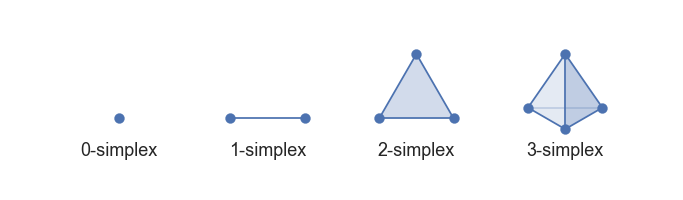
\includegraphics[width=0.5\linewidth, keepaspectratio=true]{simplices.png}
	\caption{Различные симплексы}
	\label{simplex}
\end{figure}
\begin{definition}
	Топологический симплициальный комплекс $K$ -- это множество симплексов такое, что:
	\begin{enumerate}
		\item Для каждого симплекса из $K$ его грани тоже лежат в $K$.
		\item Пересечение любых двух симплексов $\sigma, \tau \in K$ либо пусто, либо является гранью и $\sigma$, и $\tau$.
	\end{enumerate}
\end{definition}
На рисунке \ref{simplicial_complex} представлен пример симплициального комплекса. Так как среди всех симплексов, входящих в представленный на рисунке комплекс, размерность не выше $3$, то и размерность симплициального комплекса равна $3$.
\begin{figure}[!htbp]
	\centering
	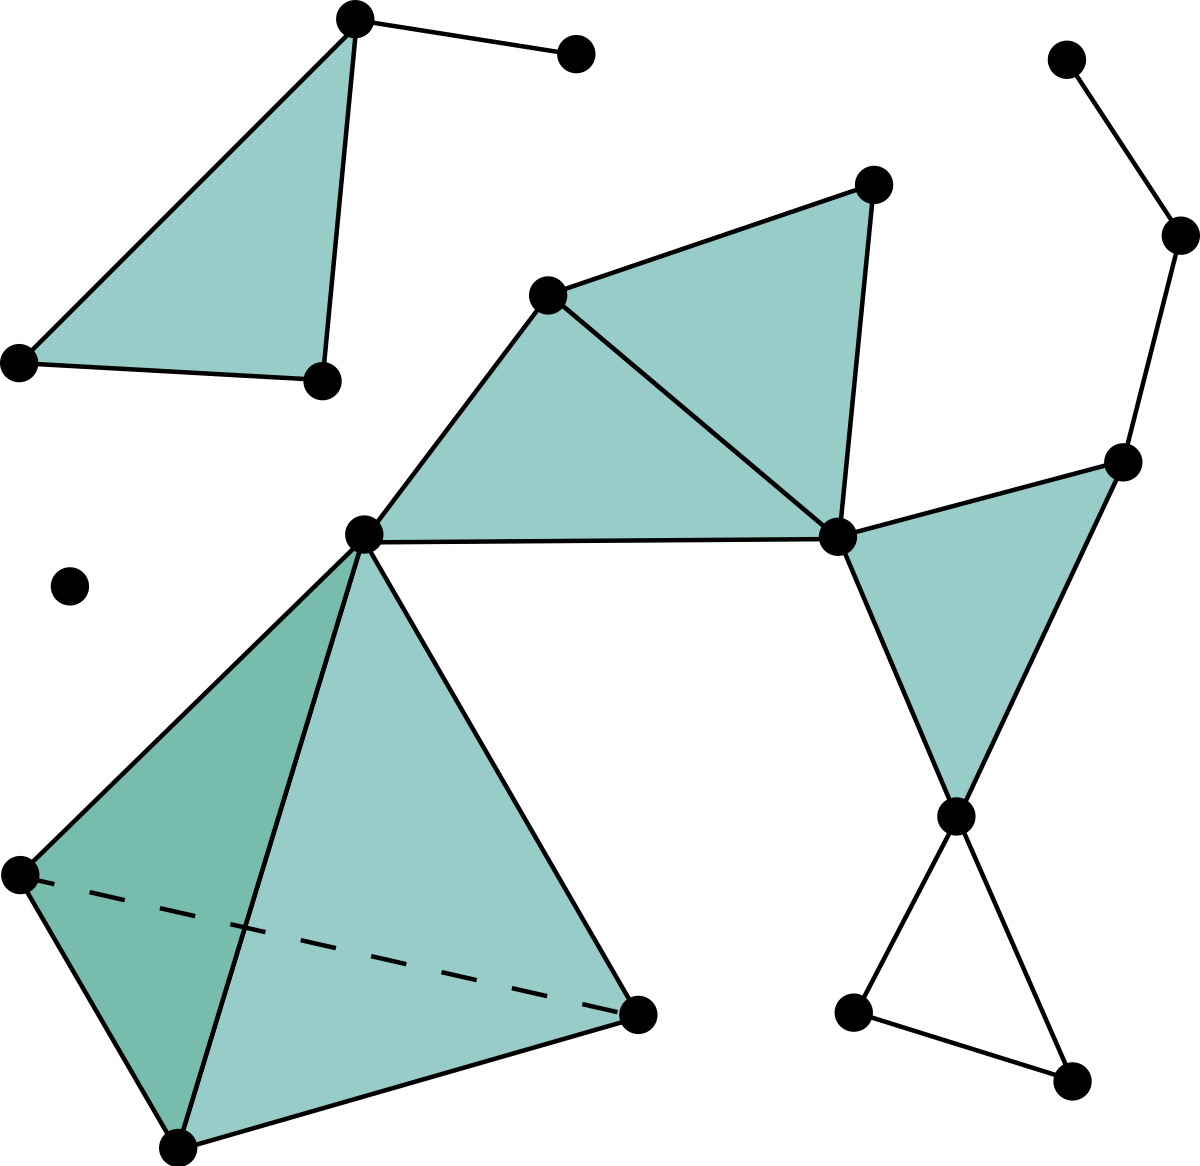
\includegraphics[width=0.5\linewidth, keepaspectratio=true]{simplicial_complex.png}
	\caption{Симплициальный комплекс}
	\label{simplicial_complex}
\end{figure}
По топологическому симплициальному комплексу можно построить топологическое пространство -- объединение его симплексов. Такие пространства тоже называют симплициальными комплексами. В таком пространстве топология индуцируется топологией на $\mathbb{R}^d$.

Имея топологическое пространство $X$, говорят, что набор его подмножеств $\{U_i : i \in J\} $ является {\it покрытием}, если $ \bigcup\limits_{i \in J} U_i = X$. Покрытие называется {\it открытым}, если оно состоит из открытых множеств.

По покрытию пространства можно построить нерв покрытия  (рисунке. \ref{nerve}) -- симплициальный комплекс, соответствующий топологическому пространству и имеющий различные интересные топологические свойства. Пусть $ [m] \coloneqq \{1, ..., m\} $ -- $m$-элементное множество.
\begin{definition}
	Нерв покрытия $N(U)$, соответствующий топологическому пространству $X$, -- это абстрактный симплициальный комплекс на $[m]$, такой что $ \{k_1, ..., k_s\} \in N(U) $ если $ U_{k_1} \cap ... \cap U_{k_s} \neq \emptyset $.
\end{definition}
\begin{figure}[h!]
	\begin{center}
		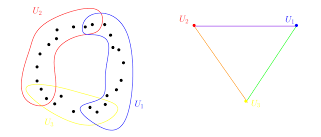
\includegraphics[width=0.75\textwidth]{nerve.png}\\
		\caption{Покрытие пространства и нерв покрытия}
		\label{nerve}
	\end{center}
\end{figure}
Если имеется 2 непрерывных отображения $f, g : X \to Y$, то говорят, что $f$ {\it гомотопно} $g$, если существует такое отображение ${H: X\times I \to Y}$, что ${H(x,0) = f}$ и ${H(x,1) = g}$. В таких случаях пишут, что ${f \sim g}$. Гомотопия является отношением эквивалентности на множестве непрерывных отображений ${ C(X,Y) }$.


Два топологических пространства $X,Y$ гомотопически эквивалентны (${X \sim Y}$), если существует такая пара ${(f,g) \in C(X,Y)^2}$, такая, что ${f \circ g \sim id_Y}$ и ${g \circ f \sim id_X}$.

С понятием нерва покрытия связана очень важная лемма:
\begin{lemma*}[о нерве]
	Если $U$ -- открытое покрытие, такое, что любое пересечение его подмножеств либо пусто, либо гомотопически эквивалентно точке, то нерв покрытия пространства $X$ гомотопически эквивалентен самому пространству
	\[ \forall I \in N(U) \left( \bigcap\limits_{i \in I} U_i = \emptyset \lor \bigcap\limits_{i \in I} U_i \sim pt \rightarrow N(U) \sim X \right). \].
\end{lemma*}

Как всякая хорошая математическая структура, симплициальные комплексы образуют {\it категорию} \cat{SCpx}. Морфизмами в такой категории являются симплициальные отображения $\varphi : M \to N$, т.е. такие отображения, что для каждого симплекса из $M$ $\varphi$ является линейным отображением на симплекс из $N$. 

Имея симплициальный комплекс, можно найти его симплициальные гомологии. Такие гомологии можно рассматривать как функтор из категории симплициальных комплексов в категорию абелевых групп: каждому симплициальному комплексу сопоставляется некоторая абелева группа. Замечательный момент заключается в том, что гомеоморфные симплициальные комплексы имеют одинаковые группы гомологий, а потому теория гомологий является очень удобным инструментом для изучения симплициальных комплексов. На самом деле данные утверждения можно легко обобщить на общий случай топологических пространств.

Дадим формальное определение симплициальным гомологиям. Итак, пусть $K$ -- симплициальный комплекс и $k\geq0$. 

{\it Группой $k\text{-цепей } C_k(K)$ симплициального комплекса $K$} называют (свободную абелеву) группу, элементами которого являются формальные суммы $k\text{-симплексов } K$, то есть
\[
c = \sum\limits_{i}\varepsilon_i\sigma_i,\;\; \varepsilon_i \in \mathbb{Z},
\] 
где конечное число $\varepsilon_i \neq 0$, $\sigma_i$ -- $k$-симплекс.
{\it Границей} $k$-цепи $\sum\limits_{i}\varepsilon_i\sigma_i$ называют $(k-1)$-цепь
\[
\partial_k(\sigma) = \sum\limits_{j=0}^{k}(-1)^j\sum\limits_{i}\varepsilon_i\partial_j\sigma_i,
\]
где $\partial_j\sigma_i = \partial_j [v_0, ..., v_k] = [v_0, ..., \hat{v_j}, ..., v_k] $ -- $(k-1)$-симплекс, порожденный всеми вершинами, кроме вершины $v_j$. Гомоморфизм $\partial_k : C_k(K) \to C_{k-1}(K)$ называют {\it граничным оператором}. Он удовлетворяет следующему свойству:
\[
\partial_{k-1} \circ \partial_k = 0.
\]	
То есть $ \im \partial_{k+1} \leq \ker \partial_k \leq C_k(K)$. Последовательность $C_k(K)$ и $\partial_k$ называется {\it цепным комплексом}

\begin{center}
	\begin{tikzcd}[cells={nodes={minimum height=2em}}]
	... \arrow[r, "\partial_{k+2}"] & C_{k+1} \arrow[r,"\partial_{k+1}"]  &  C_k \arrow[r,"\partial_k"] &  C_{k-1} \arrow[r, "\partial_{k-1}"] & ... \arrow[r, "\partial_1"] & C_0.
	\end{tikzcd}
\end{center}

Цепной комплекс можно визуализировать следующим образом (рисунок \ref{chain}).

\begin{figure}[!htbp]
	\centering
	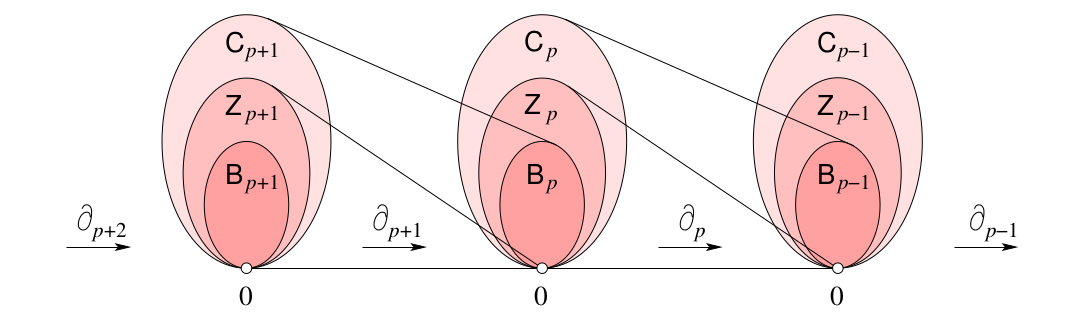
\includegraphics[width=0.5\linewidth, keepaspectratio=true]{chain.png}
	\caption{Цепной комплекс}
	\label{chain}
\end{figure}

\begin{definition}
	$k$-ой группой гомологий симплициального комплекса $K$ называют следующее фактор-пространство:
	\[
	H_k(K) = \quotient{\ker \partial_k}{\im \partial_{k+1}}.
	\]
	
	Тогда $k$-ое число Бетти -- размерность $k$-ой группы гомологий: 
	\[\beta_k(K) = \dim H_k(K).\] 
\end{definition}

При $k=0$ число Бетти описывает количество компонент связности данного пространства. При $k=1$ -- количество циклов. При $k=2$ число Бетти описывает количество  <<полостей>>. В таблице \ref{tabl:betti} представлены первые числа Бетти для некоторых пространств.

\begin{center}
	\begin{table}[!htbp]
		\centering
		\caption{Первые числа Бетти для некоторых пространств}
		\begin{tabular}{ |c|c c c| }
			\hline
			Пространство & $\beta_0$ & $\beta_1$ & $\beta_2$ \\ 
			\hline
			Pt & 1 & 0 & 0 \\ 
			$D^2$ & 1 & 0 & 0 \\ 
			Треугольник & 1 & 0 & 0 \\
			Граница треугольника & 1 & 1 & 0 \\
			$S^1$ & 1 & 1 & 0 \\
			$S^2$ & 1 & 0 & 1 \\
			$\mathbb{T}^2 = S^1 \times S^1$ & 1 & 2 & 1 \\
			\hline
		\end{tabular}
		\label{tabl:betti}
	\end{table}
\end{center}


\section{Персистентные гомологии и их векторные представления}
\subsection{Персистентные гомологии}
Далее будет приведен теоретический материал по устойчивым гомологиям. Подробнее можно прочитать в \cite{Edelsbrunner, base, alsobase}

О персистентных(устойчивых) гомологиях можно думать как об адаптации понятия гомологии к облаку точек. 

Имея облако точек $X$, существует много способов построения симплициальных комплексов по нему. Например, задав некоторый $\tau > 0$, можно рассматривать не просто точки, но и их окрестности с радиусом $\tau$. Тогда можно рассматривать следующую структуру: подмножество $\sigma \subset X$ будет симплексом, если пересечение окрестностей точек из $\sigma$ будет непусто. Тогда симплициальным комплексом, построенным по облаку точек, будет совокупность таких симплексов. Такой симплициальный комплекс называется \text{\it комплексом Чеха} $\Cech_\tau(X)$. 

На комплекс Чеха можно взглянуть с другой стороны: если данные действительно хорошо описывают некоторый топологический объект, который как бы стоит за этими данными, то, подобрав хороший радиус $\tau$, объединение полученных окрестностей будет гомотопически эквивалентно этому объекту. А так как все шары выпуклы, то объединение окрестностей будет гомотопически эквивалентно нерву данного покрытия. А значит, по лемме о нерве, сам нерв будет гомотопически эквивалентен топологическому объекту, который описывается данными. И комплекс Чеха как раз и является нервом покрытия. 

Но на практике оказывается, что комплекс Чеха очень сложно посчитать. Поэтому существует другой способ построения симплициального комплекса по облаку точек, более эффективный с точки зрения вычислений: зафиксировав $\tau$, подмножество $\sigma \subset X$ будет симплексом, если $\forall i,j \in \sigma: \rho(i,j) < \tau$. Симплициальным комплексом будет совокупность таких симплексов. Полученный симплициальный комплекс называется \text{\it комплексом Вьеториса—Рипса}(или просто {\it комплексом Рипса}) $\Rips_\tau(X)$.

\medskip
\begin{algorithm}[H]
	\small
	\SetAlgoLined
	\KwData{Облако точек $X$, вещественное число $\alpha > 0$. }
	\KwResult{Симплициальный комплекс Вьеториса—Рипса}
	Для каждой точки $x$ строим её $\alpha$-окрестность $B_\alpha(x)$;
	
	$i = 1$;
	
	\While{$i+1$ окрестностей попарно имеют непустое пересечение}{
		
		строим $i$-ый симплекс на соответствующих вершинах;
		
		$i \leftarrow i+1$; 
	}
	\caption{Алгоритм построения комплекса Вьеториса—Рипса}
\end{algorithm}
\medskip

То есть, вместо рассмотрения пересечений шаров, как это было в случае комплекса Чеха, рассматривают попарные расстояния между точками. Очевидно, такой подход более эффективен с вычислительной точки зрения, более того, его можно обобщить на общий случай конечного метрического пространства, и даже, более общо, на случай произвольного конечного множества с симметрической функцией.

Комплексы Чеха и Рипса связаны между собой: для облака точек $X \subset \mathbb{R}^d$ они имеют одинаковый 1-остов. Более того, справедливо следующее соотношение:
\[
	\Rips_\tau(X) \subseteq \Cech_\tau(X) \subseteq \Rips_{2\tau}(X).
\]

На рис. \ref{complexes} изображены комплексы Чеха и Рипса.

\begin{figure}[!htbp]
	\begin{center}
		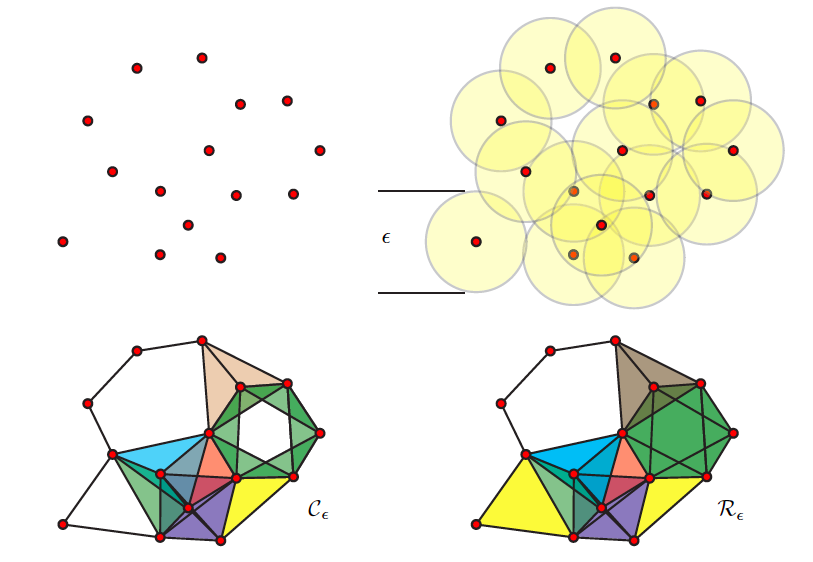
\includegraphics[width=0.75\textwidth]{complexes.png}\\
		\caption{Комплексы Чеха и Вьеториса—Рипса}
		\label{complexes}
	\end{center}
\end{figure}

Везде выше параметр $\tau$ был зафиксирован, но его можно изменять. Вслед за этим будут меняться и симплициальные комплексы, построенные с учетом $\tau$. {\it Фильтрацией симплициального комплекса $K$} называют вложенное семейство подкомплексов $ (K_\tau)_{\tau \in T} $, где $ T \subseteq \mathbb{R} $, такое, что если $ \tau < \tau^{'} $, то $ K_\tau \subseteq K_{\tau^{'}} $. Пример такой фильтрации изображен на рис. \ref{ripsfilt}, где изображения фильтрация симплициальных комплексов Рипса $\Rips_\tau(X)$.

\begin{figure}[!htbp]
	\begin{center}
		
\includegraphics[width=0.75\textwidth]{filtration.png}\\
		\caption{Фильтрация Рипса}
		\label{ripsfilt}
	\end{center}
\end{figure}

Имея фильтрацию $(K_\tau)_{\tau \in T}$, можно отслеживать изменение $H_k(K_\tau)$ с ростом $\tau$: могут появляться новые компоненты связности, уже существующие могут объединяться в одну компоненту, могут появляться циклы и "пустоты", соответствующие $1$ и $2$ группе гомологий. 
\begin{definition}
	$k$-ыми устойчивыми гомологиями фильтрованного комплекса $ (K_\tau)_{\tau \in T} $ называют  проиндексированное семейство абелевых групп $H_n(T) = \{ (H_n(K_\tau))_{\tau \in T} $ вместе с семейством гомоморфизмов $ (H_n(K_\tau) \to H_n(K_\tau^{'}))_{\tau \leq \tau^{'}} \}$.
\end{definition}
Такое семейство абелевых групп вместе с морфизмами на самом деле является примером  персистентного $\mathbb{Z}$-модуля($\mathbb{Z}$-модуля устойчивости): {\it персистентным $R$-модулем} $(A_*, x) $ называют последовательность $R$-модулей и гомоморфизмов между ними (над целочисленной временной шкалой $\mathbb{Z}_{\geq0}$).
\begin{center}
	\begin{tikzcd}[cells={nodes={minimum height=2em}}]
	A_0 \arrow[r, "x"] & A_1 \arrow[r,"x"]  &  A_2 \arrow[r,"x"] &  A_3 \arrow[r, "x"] & ... 
	\end{tikzcd}
\end{center}
Основная теорема про персистентные модули -- это структурная теорема. По аналогии с обычными модулями, она формулируется в терминах {\it конечнопорожденного} модуля устойчивости, т.е. такого модуля $(A_*, x)$, у которого существует конечный набор $a_1, ..., a_k \in A_*$ элементов, что любой элемент $a \in A_*$ можно выразить в виде линейной комбинации элементов вида $x^sa_r = x \circ ... \circ x(a_r)$.  Для ее формулировки понадобится еще пару определений: если $0 \leq j < s$, то {\it интервальным модулем устойчивости $I_{[j,s)}$} называют модуль устойчивости вида
\begin{center}
	\begin{tikzcd}[cells={nodes={minimum height=2em}}]
	0 \arrow[r] & ... \arrow[r]  &  0 \arrow[r] &  \underset{j}{R} \arrow[r, "id_R"] &  \underset{j+1}{R} \arrow[r, "id_R"] &
	... \arrow[r, "id_R"] & \underset{s-1}{R} \arrow[r, "0"] & \underset{s}{0} \arrow[r] & ... 
	\end{tikzcd}
\end{center}
Аналогично определяется бесконечный интервальный модуль $I_{[j, \infty)}$
\begin{center}
	\begin{tikzcd}[cells={nodes={minimum height=2em}}]
	0 \arrow[r] & ... \arrow[r]  &  0 \arrow[r] &  \underset{j}{R} \arrow[r, "id_R"] &  \underset{j+1}{R} \arrow[r, "id_R"] &
	... \arrow[r, "id_R"] & R \arrow[r, "id_R"] &  ... 
	\end{tikzcd}
\end{center}
Можно определить прямую сумму персистентных модулей: $ (A_*, x) \oplus (B_*, x) = ((A_* \oplus B_*), x) $, где $(A_* \oplus B_*)_j = A_j \oplus B_j$, а $x$ действует на каждом из слагаемых по отдельности.
\begin{theorem*}[об интервальном разложении] Пусть $R$ -- произвольное поле, а $(A_*, x)$ -- конечнопорожденный персистентный $R$-модуль. Тогда $(A_*, x)$ имеет единственное с точностью до перестановки слагаемых представление в виде прямой суммы конечного числа интервальный модулей:
	\[
		(A_*, x) \simeq \big( \bigoplus\limits_{k} I_{[j_k, s_k]} \big) 
																		\oplus 
						\big( \bigoplus\limits_{k} I_{[r_k, \infty)} \big)
	\]
\end{theorem*}

Так как персистентные гомологии -- это типичный пример конечнопорожденного персистентного модуля, то к нему можно применить структурную теорему. Из теоремы следует, что любой конечнопорожденный персистентный модуль с коэффициентами в поле, а значит и персистентные гомологии, можно закодировать в виде баркода (рис. \ref{barcode}) -- диаграммы, которая содержит интервалы, которые отвечают за время жизни свойств, которые как раз и характеризуются персистентными гомологиями.
\begin{figure}[]
	\begin{center}
		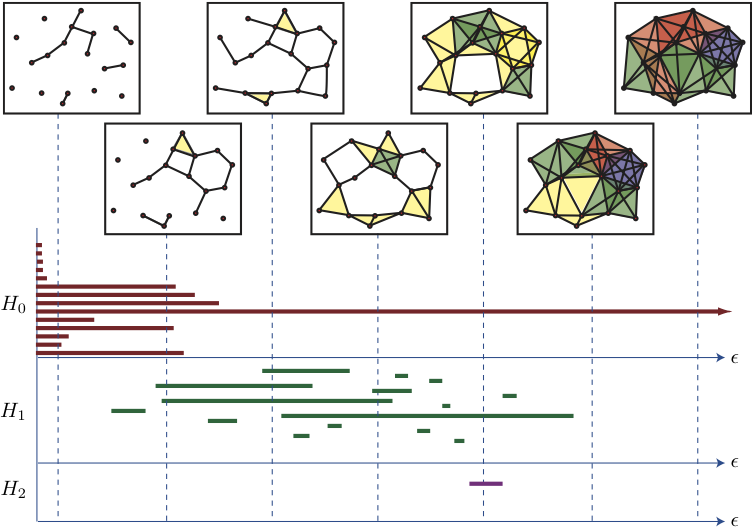
\includegraphics[width=0.75\textwidth]{barcode.png}\\
		\caption{Баркод}
		%\emph{Рис. 2. Баркод}
		\label{barcode}
	\end{center}
\end{figure}
\newline
Эту же информацию можно закодировать в виде диаграммы персистентности(диаграммы устойчивости) (рис. \ref{persist_diag}). Она строится следующим образом: каждый интервал баркода имеет начало $t_{birth}$ и конец $t_{death}$. На персистентной диаграмме каждый интервал баркода изображается в виде точки с координатами ($t_{birth}, t_{death}$), и каждая такая точка соответствует одному из слагаемых $I_{[j_k, s_k]}$ и $I_{[r_k, \infty)} $ из разложения. Таким образом, диаграмма устойчивости $B$ -- это множество $\{ (x,y) \in \mathbb{R} \times \mathbb{R} \cup \infty | x \leq y\}$. Чем дальше точка на персистентной диаграмме от диагонали, тем она важнее -- эта точка сигнализирует о наличии "$n$-мерной дырки". 
\begin{figure}[]
	\begin{center}
		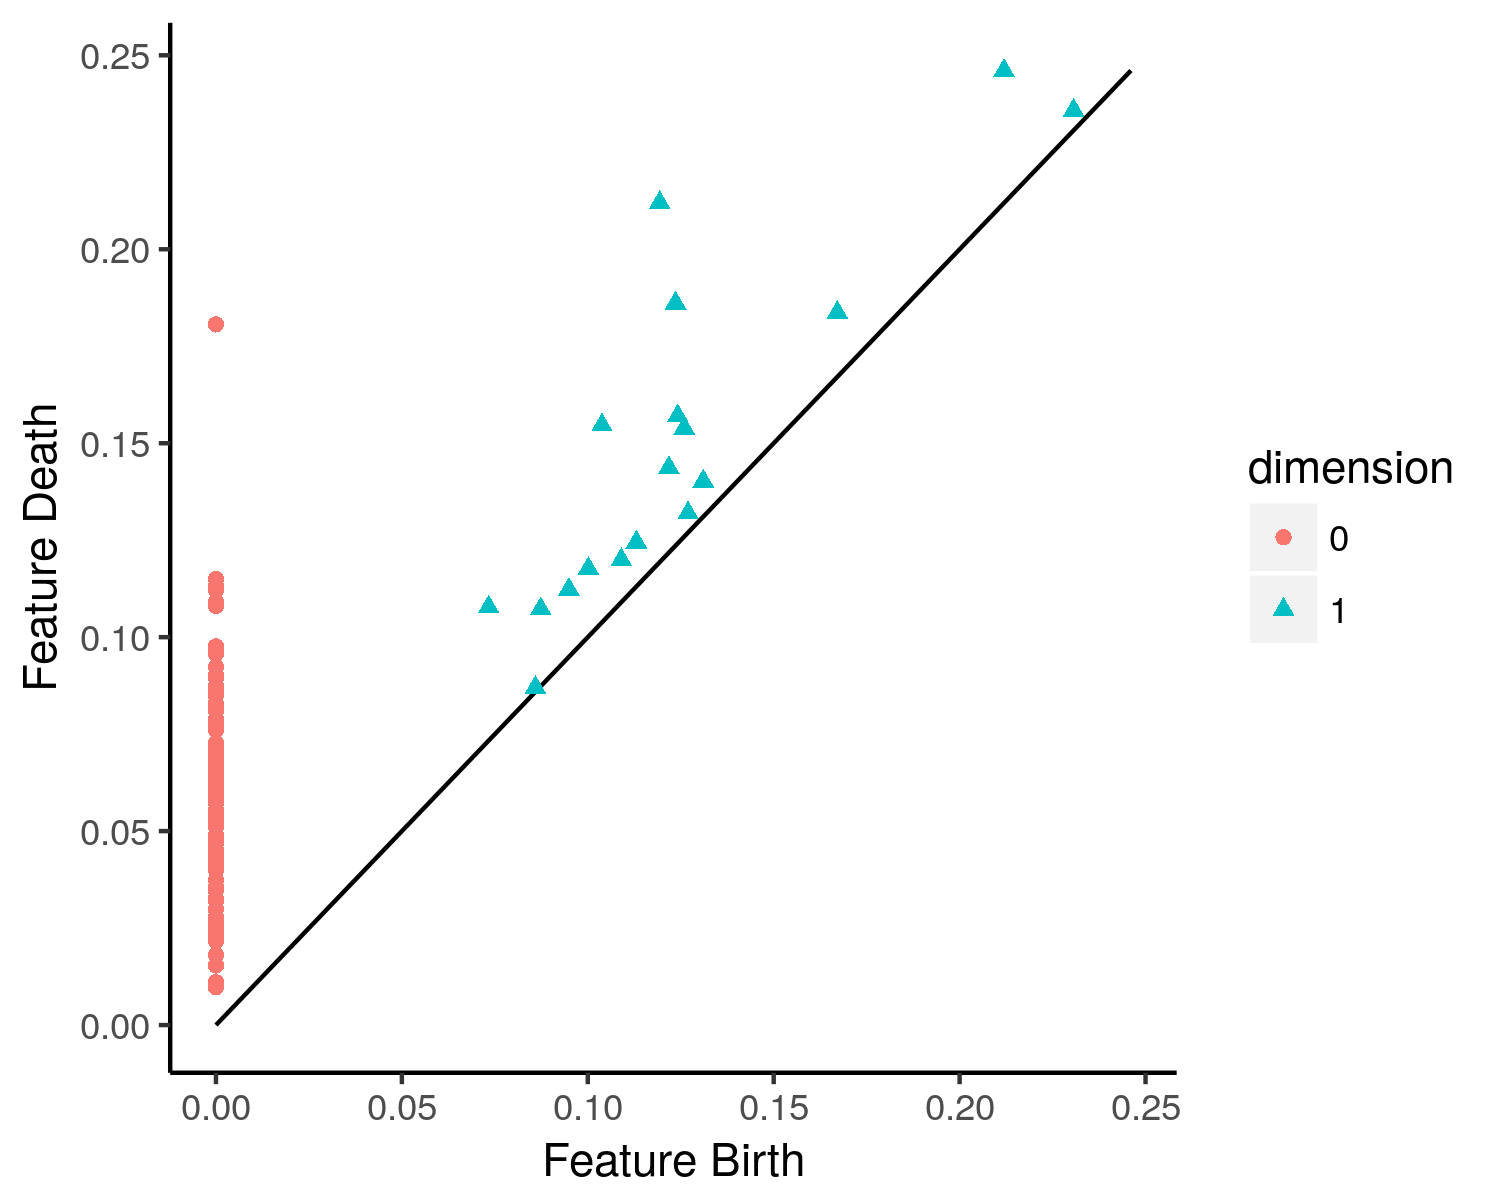
\includegraphics[width=0.75\textwidth]{persist_diag.png}\\
		\caption{Персистентная диаграмма}
		%\emph{Рис. 3. Персистентная диаграмма}
		\label{persist_diag}
	\end{center}
\end{figure}

\subsection{Векторные представления}
Как было показано выше, диаграмма устойчивости кодирует топологическую информацию. Кажется естественным, что такую топологическую информацию можно использовать во многих задачах анализа данных и машинного обучения. Однако для этого необходимо что-то знать про множество всех устойчивых диаграмм.

Пусть $\mathcal{D}$ -- множество устойчивых диаграмм. На нем можно ввести (естественную) метрику:
\[
W_p(B, B^{'}) = \inf\limits_{\gamma:B\to B^{'}} 
\big( 
\sum\limits_{u \in B} \norm{u - \gamma(u)}_\infty^p
\big) ^{\frac{1}{p}},
\]
где где $1 \leq p < \infty$, $B, B^{'}$ -- диаграммы персистентности. Такую метрику называют {\it $p-$метрику Васерштейна}. Другой естественной метрикой является т.н. {\it bottleneck distance} $W_\infty$:
\[
W_\infty(B, B^{'}) = \inf\limits_{\gamma:B\to B^{'}} \sup\limits_{u \in B}
\norm{u - \gamma(u)}_\infty.
\]
Таким образом, $\mathcal{D}$ с любой из указанных выше метрик образует метрическое пространство. 

Несложно увидеть, что, к сожалению, оно не является полным: пусть $x_n = (0, 2^{-n}) \in \mathbb{R}^2$ и $B_n = \{x_i\}_{i=1}^n$ -- диаграмма устойчивости. Тогда
\[
	W_p(B_n, B_{n+k}) \leq \frac{1}{2^{n+k}},
\]
а значит $\{B_n\}$ фундаментальна. Однако при $n \to \infty$ число недиагональных элементов в $B_n$ уходит в бесконечность, поэтому у последовательности диаграмм нет предела. 

Можно немного изменить определение устойчивых диаграмм -- пусть теперь у нас всегда она содержит диагональ $\Delta = \{(x,y) \in \mathbb{R}^2 | x=y\}$. Для таких диаграмм $p$-метрика Васерштейна обобщается естественным способом. Пустую диаграмму, содержащую только диагональ, будем обозначать через $B_\emptyset$. Тогда пространством устойчивых диаграмм можно считать следующее пространство:
\[
	\mathcal{D} \{ B | W_p(B, B_\emptyset) \textless \infty \}.
\]
Тогда, как показано в \cite{prop_measures}, такое пространство уже обладает хорошими свойствами, например оно полно и сепарабельно.

Однако для большинства алгоритмов машинного обучения и анализа данных этого недостаточно. Например, для метода опорных векторов необходимо, чтобы пространство признаков было гильбертовым(например, евклидовым), т.к. такой метод строит разделяющую гиперплоскость; деревья решений строят иерархическую модель "решений", которые, в свою очередь, также определяют гиперплоскость. 

Более того, в пространстве $\mathcal{D}$ устойчивых диаграмм, как также было показано в \cite{prop_measures}, даже такая стандартная статистика, как среднее арифметическое, для диаграмм устойчивости можно по-разному считать и интерпретировать. Например, если одна диаграмма, $B_1$, содержит 2 точки $B_1 = \{ (10, 22), (12, 20) \}$, а вторая диаграмма, $B_2$, содержит другие две точки $B_2 = \{ (10, 22), (12, 20) \}$, то что считать средним? Диаграмму $ \{ (11, 20), (11, 22) \}$ или $\{ (10,21), (12,21) \}$? Аналогичная ситуация обстоит и с дисперсией. 

Таким образом, геометрия пространства $\mathcal{D}$ персистентных диаграмм не позволяет комфортно с ними работать. Значит, для того, чтобы использовать диаграммы устойчивости в анализе данных и машинном обучении, нужно каким-то образом преобразовывать исходное пространство $\mathcal{D}$ диаграмм устойчивости в подходящее, например, гильбертово. Для этого существует несколько подходов. Далее опишем только те, что будут использоваться в данной работе -- это betti curves, persistent landscapes и heat kernel.

Итак, пусть $B = \{ (b_i, d_i) \}_{i=1}^n$ -- диаграмма персистентности. Тогда ее {\it Betti curve} назовем функцию $\beta_B: \mathbb{R} \to \mathbb{N} : t \mapsto \abs{\{(b_i, d_i) | b_i \le t \textless d_i\}}$. Иногда ее называют как persistence indicator function(PIF). Такие функции являются на самом деле ступенчатыми функциями, а потому образуют векторное пространство: суммой таких двух функций $\beta_B + \beta_C \coloneqq \beta_{B \cup C}$. На рис. \ref{betti-curve} показан график такой функции.

\begin{figure}[]
	\begin{center}
		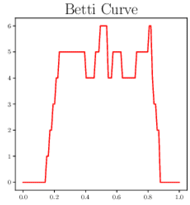
\includegraphics[width=0.3\textwidth]{betti-curve.png}\\
		\caption{График Betti curve}
		\label{betti-curve}
	\end{center}
\end{figure}

Как было показано выше, в пространстве персистентных диаграмм среднее не единственно. Но у Betti curve такой проблемы нет: для набора $\beta_1, ..., \beta_N$ Betti curves для устойчивых диаграмм $B_1, ..., B_N$ среднее $\bar\beta$ можно определить покомпонентно:
\[
	\bar\beta(t) = \frac{1}{N}\sum\limits_{i=1}^{N} \beta_i(t).
\]

В \cite{PIF} показано, что Betti curve устойчива относительно нормы $\norm{\beta}_1 = \int\limits_{\mathbb{R}} \abs{\beta(t)}dt$. Это означает, что небольшие изменения диаграммы приводят к небольшим изменениям Betti curve.

Пусть, все так же, $B = \{ (b_i, d_i) \}_{i=1}^n$ -- диаграмма персистентности. Тогда для каждой пары $(b_i, d_i)$ можно определить кусочно-линейную функцию $f_{(b_i, d_i)}: \mathbb{R} \to [0, \infty]$:
\[
	f_{(b_i, d_i)} : x \mapsto
	\left\{
		\begin{array}{ll}
			0, & \text{если } x \notin (b_i, d_i), \\
			x - b_i, & \text{если } x \in (b_i, \frac{b_i + d_i}{2}), \\
			-x + d, & \text{если } x \in (\frac{b+d}{2}, d)
		\end{array}
	\right.
\]
Тогда {\it persistent landscapes} диаграммы устойчивости $B$ -- это последовательность функций $\lambda_k : \mathbb{R} \to [0, \infty]$, где $k=1, 2, 3, ...$, и где $\lambda_k(x)$ -- это $k$-ое наибольшее значение последовательности $\{f_{(b_i, d_i)}(x)\}_{i=1}^n$, а если такого значения нет, то $\lambda_k=0$. Эквивалентно, можно определить persistent landscape как функцию $\lambda: \mathbb{N} \times \mathbb{R} \to [0, \infty]: (k,t) \mapsto \lambda_k(t)$. На рис. \ref{persist_land} представлен пример такого представления.

\begin{figure}[]
	\begin{center}
		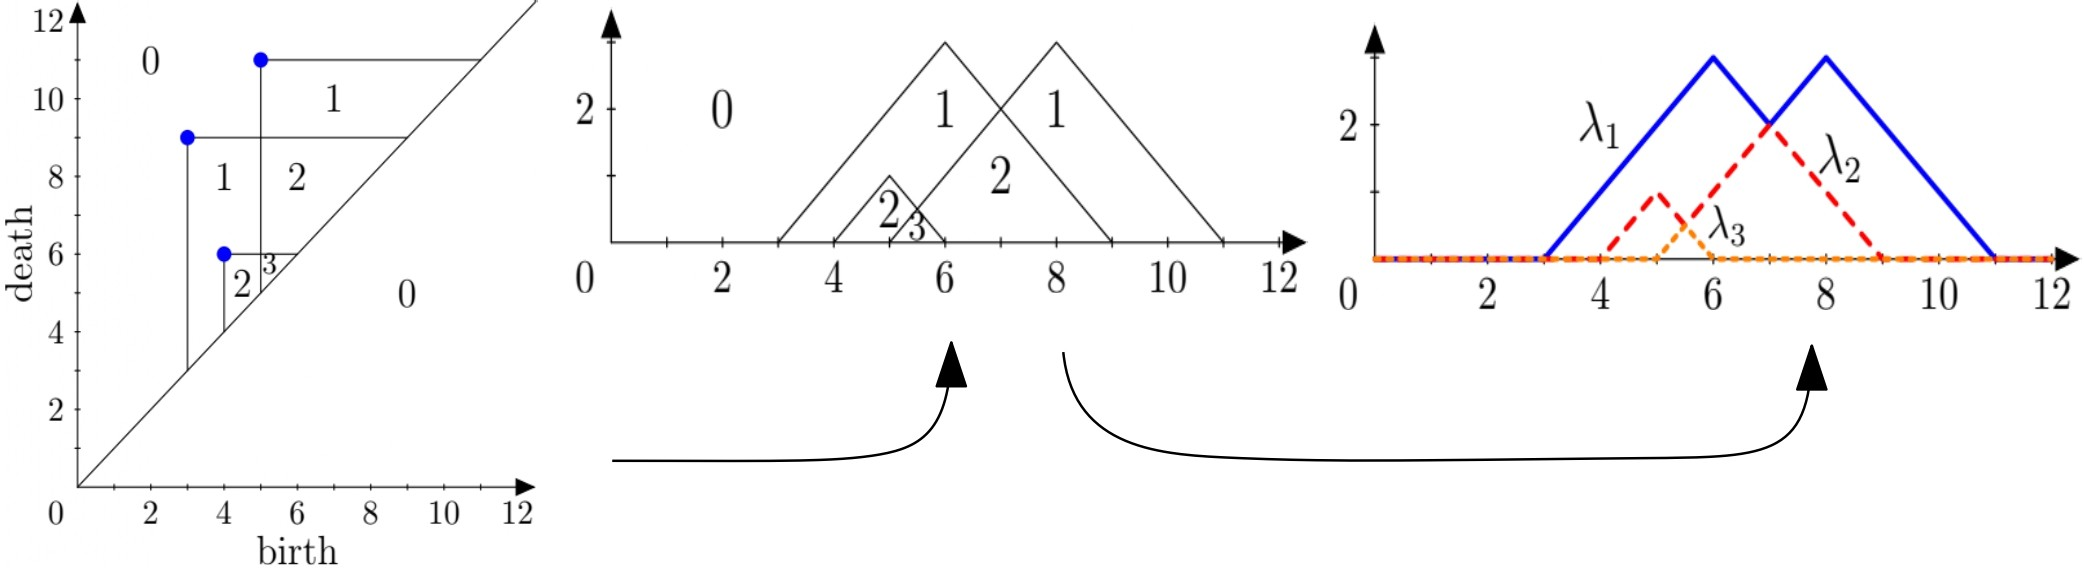
\includegraphics[width=0.75\textwidth]{persistent_landscape.jpeg}\\
		\caption{График persistent landscape}
		\label{persist_land}
	\end{center}
\end{figure}

Также как и Betti curves, для persistent landscapes можно посчитать среднее: пусть $\lambda^1, ..., \lambda^N$ -- persistent landscapes для $B_1, ..., B_N$ диаграмм. Тогда их среднее, $\bar\lambda$ можно определить покомпонентно:
\[
	\bar\lambda_k(t) \coloneqq \frac{1}{N}\sum\limits_{i=1}^{N} \lambda_k^i(t).
\]

Между persistent landscapes можно посчитать расстояние, например, используя $L^p$ норму:
\[
	\norm{\lambda - \lambda^{'}}_p = \big( \sum\limits_{k=1}^{\infty} \int \abs{ \lambda_k(t) - \lambda_k^{'}(t) }^p dt \big)^{\frac{1}{p}}.
\]

В \cite{pers_land} показано, что persistent landscape устойчива относительно метрики $L^p$ для $1 \le p \le \infty$. Это означает, что небольшие изменения диаграммы приводят к небольшим изменениям persistent landscape. 

Также рассматриваем $B = \{ (b_i, d_i) \}_{i=1}^n$ -- диаграмму персистентности. Определим для нее heat kernel. Напомним, что если $X$ -- некоторое множество, то функция $k: X \times X \to \mathbb{R}$ является {\it ядром(kernel)}, если существует Гильбертово пространство $\mathcal{H}$ и отображение(т.н. feature map) $\Phi:X \to \mathcal{H}$, такое, что $\forall x, y$ имеет место $k(x,y) = \langle \Phi(x), \Phi(y) \rangle_\mathcal{H}$, т.е. следующая диаграмма коммутативна:

\[
\begin{tikzcd}
&X \arrow[rr,"\Phi"] &[-1.5em] &[-1.5em] H \\
X \times X \arrow[dr,"\pi_X"'] \arrow[ur,"\pi_X"] \arrow[rr,"k"] &&
\mathbb{R} &&
\mathcal{H} \times \mathcal{H} \arrow[ul,"\pi_\mathcal{H}"']
\arrow[dl,"\pi_\mathcal{H}"] \arrow[ll,"{\langle \cdot, \cdot \rangle_\mathcal{H}}"'] \\
&X \arrow[rr,"\Phi"] && H
\end{tikzcd}
\]

Заметим, что диаграмма устойчивости $B$ можно единственным образом сопоставить сумму распределений дельта-функций Дирака в каждой точке диаграммы. Такой взгляд на диаграмму устойчивости позволяет каноническим образом получить структуру Гильбертова пространства. Тогда для данной диаграммы устойчивости $B$ можно рассмотреть следующее уравнение теплопроводности с граничным условием Дирихле:
\[
\begin{array}{ll}
	\Delta_x u = \partial_t u, & (x,t) \in \mathrm{Int}(\Omega \times \mathbb{R}_{\geq 0}), \\
	u = 0, & (x,t) \in \partial\Omega \times \mathbb{R}_{\geq 0}), \\
	u = \sum\limits_{x \in B} \delta_x, & (x,t) \in \Omega \times \{0\},
\end{array}
\]
где $\delta_x$ -- дельта-функция Дирака в точке $x$, а $\Omega = \{ (x_1, x_2) | x_1 \leq x_2 \} \subset \mathbb{R}^2$. Тогда решение данного уравнения -- функция в $L_2(\Omega)$, а значит можно рассмотреть отображение $F_\sigma: \mathcal{D} \to L_2(\Omega): B \mapsto \restr{u}{t=\sigma}$. Заметим, что $F_\sigma$ инъективно. Таким образом, можно определить ядро $k_\sigma: \mathcal{D} \times \mathcal{D} \to \mathbb{R}: (B, C) \mapsto \langle \Phi_\sigma(B), \Phi_\sigma(C) \rangle_{L_2(\Omega)}$. В \cite{heat_kernel} приведена мотивация построения именно такого ядра. также в \cite{heat_kernel} показано, что $k_\sigma$ устойчива относительно $1-$ метрики Васерштейна.

Все описанные выше методы сопоставляют диаграмме устойчивости некоторую функцию в Банаховом пространстве. Эти методы являются примерами векторизации. {\it Векторизацией} на множестве $X$ называют отображение $\varphi: X \to V$, где $V$ -- векторное пространство. Имея такую векторизацию, можно определить {\it амплитуду}: отображение $A: X \to \mathbb{R}: x \mapsto \norm{\varphi(x)}$, где $\varphi: X \to V$ -- векторизация множества $X$ на нормированное векторное пространство. Таким образом, для каждой диаграммы, выбрав определенную векторизацию, можно получить ее амплитуду, т.е. каждой диаграмме сопоставить некоторое вещественное число. Другой способ это сделать -- это посчитать т.н. {\it персистентную энтропию} -- это мера энтропии по Шеннону точек на диаграмме персистентности:
\[
E(B) = - \sum\limits_{i \in I} p_i \log(p_i), \text{ где $p_i = \dfrac{d_i - b_i}{\sum\limits_{i \in I}d_i-b_i}$. }
\]

Более подробно с персистентной энтропией можно ознакомиться в \cite{pers-entr}. Тогда, получив такие значения, из них можно сделать вектор в $\mathbb{R}^d$, который будет соответствовать диаграмме устойчивости. Такой вектор уже можно будет использовать в задачах анализа данных и машинного обучения.

\section{\centering Элементы машинного обучения} 
Здесь будут приведены некоторые теоретические сведения из анализа данных и машинного обучения. За более подробным материалом можно обратиться к \cite{bishop, mathforml, ml-coursera}.

\subsection{\centering Введение в машинное обучение}
{\it Машинное обучение} -- раздел, стоящий на пересечении математики и компьютерных наук, который, главным образом, решает задачу восстановления некоторой зависимости, используя некоторые данные, которые представляют такую зависимость. 

Машинное обучение можно разделить на категории: например, очень популярное разделение -- это разделение по типу обучения:
\begin{itemize}
	\item обучение с учителем(Supervised Learning);
	\item обучение без учителя(Unsupervised Learning);
	\item обучение с подкреплением(Reinforcement Learning).
\end{itemize}

Остановимся более подробно на обучении с учителем. Данный вид машинного обучения предполагает, что имеется некоторая выборка $X$ -- {\it множество объектов}, некоторая выборка $Y$ -- {\it множество ответов}, и необходимо восстановить {\it скрытую зависимость} $y: X \to Y$. Как правило, саму зависимость восстановить порой очень трудно, поэтому достаточно найти такой алгоритм $a: X \to Y$, который приближает $y$ на $X$. При этом сами объекты задаются через {\it признаки} $f: X \to D$, где $D$ -- {\it пространство признаков}. Признаки -- это какие-либо характеристики, которые описывают данный объект. 

Основные задачи обучения с учителем:
\begin{itemize}
	\item регрессия;
	\item классификация.
\end{itemize}

Фундаментальная разница между этими двумя типами задач следующая: задача {\it регрессии} -- восстановление непрерывной функции, которая характеризует скрытую зависимость между входными переменными и выходными. Регрессия таким имеет возможность предсказывать численное значение этой скрытой непрерывной функции по новым значениям входных переменных. Задача {\it классификации} же в том, чтобы восстановить зависимость между входными параметрами, описывающие объект, и тем, к какому классу данный объект принадлежит. То есть в случае задачи классификации скрытая зависимость описывается некоторой пороговой функцией, где каждое значение области значения соответствует некоторому классу.

Важным шагом в решении задачи как регрессии, так и классификации, является выбор модели и настройка ее параметров. {\it Модель} -- это параметрическое семейство функций 
\[
	A \coloneqq \{ a(x) = g(x, \theta) | \theta \in \Theta \},
\]
где $\Theta$ -- множество значений параметра $\theta$, а $g: X \times \Theta \to Y$ -- некоторая фиксированная функция.

Решение задачи машинного обучения разделяется на два этапа:
\begin{enumerate}
	\item этап обучения;
	\item этап применения.
\end{enumerate}

Этап обучения представляет из себя построение алгоритма выбора подходящей модели, т.е. имеется отображение $\mu: X \times Y \to A$, которое по каждой выборке $(X,Y)$, которую обычно называют {\it обучающей выборкой}, ставит в соответствие алгоритм $a \coloneqq \mu(X, Y)$, который наилучшим образом описывает скрытую зависимость $y: X \to Y$. Для выбора модели необходимо сравнивать точность, которую они демонстрируют. Для этого обычно вводят т.н. {\it функцию потерь (loss function)} $L(a,x)$, которая измеряет величину ошибки алгоритма $a \in A$ на объекте $x \in X$. Например, для задачи классификации рассматривают {\it индикатор ошибки (Accuracy)}:
\[
	L(a,y,x) = [a(x) \neq y(x)].
\]

Для задач регрессии в качестве функции потерь рассматривают {\it квадратичную ошибку} 
\[
	L(a,y,x) = (a(x) - y(x))^2
\]
или {\it абсолютное значение ошибки}
\[
	L(a,y,x) = \abs{a(x) - y(x)}.
\]

Чтобы оценить качество работы алгоритма $a$ на всей выборке $X$ обычно считают среднее арифметическое по значениям функции потерь для каждого объекта $x \in X$(иногда его называют {\it эмпирическим риском}):
\[
	Q(a,X, Y) = \frac{1}{\abs{X}}\sum\limits_{i=1}^{\abs{X}} L(a,y_i, x_i).
\]
И тогда для выбора модели решают задачу минимизации эмпирического риска:
\[
	\mu(X, Y) = \arg\min\limits_{a \in A} Q(a, X, Y).
\]


Этап применения -- это следующий этап, который представляет собой т.н. задачу вывода. На этом этапе выбранный алгоритм $a$ для новых объектов $X^*$, которые не были задействованы в этапе обучения, выдает ответы $a(X^*)$. Обычно такую выборку $X^*$ называют {\it тестовой выборкой}. Одна из основных проблем, которая возникает на данном этапе -- это проблема {\it переобучения}. Переобучение -- это ситуация, которая возникает в следствие допущенной ошибки в ходе этапа обучения, и характеризуется тем, что величина ошибки на тестовой выборке сильно превышает величину ошибки на обучающей:
\[
	Q(\mu(X, Y), X^*, Y^*) >> Q(\mu(X, Y), X, Y).
\]
Зачастую такую проблему можно исправить, если правильно подобрать параметры модели, которая использовалась для обучения.

Так как данная работа представляет собой решение задачи классификации, то остановимся поподробнее на соответствующих моделях машинного обучения.

\subsection{\centering Логистическая регрессия}
Логистическая регрессия -- один из самых простых и популярных алгоритмов для задачи классификации. Смысл данного метода заключается в том, чтобы построить разделяющую гиперплоскость в пространстве признаков, позволяющую отделить классы друг от друга. 
\newline
В логистической регрессии строится линейный алгоритм классификации $ a:X \to Y $, где $X$ -- пространство признаков, а $Y$ -- конечное множество номеров классов. Алгоритм имеет вид:
\[
a(x,w) = sign(\sum_{j=1}^{n}w_jf_j(x)-w_0) = sign\langle x,w\rangle,
\]
где $w$ -- вектор весов, $w_0$ -- порог принятия решения, а $ \langle \cdot, \cdot \rangle $ -- скалярное произведение.
\newline
Задача обучения линейного классификатора заключается в том, чтобы по выборке настроить вектор весов. Для этого в логистической регрессии решается задача минимизации эмпирического риска с специальной функцией потерь вида:
\[
Q(w) = \sum_{i=1}^{m}ln(1+e^{-y_i\langle x_i,w\rangle}) \to \min_{w}
\]
После нахождения решения $w$, становится возможным не только вычислять классификацию для произвольного объекта, но и оценивать апостериорные вероятности его принадлежности классам:
\[
\mathbb{P}(y|x) = \sigma(y\langle x,w\rangle)
\]
где $\sigma(z) = \frac{1}{1+e^{-z}}$ -- сигмоидная функция.


\subsection{\centering Метод опорных векторов}
Метод опорных векторов -- также очень популярный метод машинного обучения, достаточно мощный и многогранный, применяемый в задачах классификации и регрессии. 
\newline
Фундаментальная идея метода опорных векторов заключается в поиске гиперплоскости с наилучшим отступом -- расстоянием между гиперплоскостью и опорными векторами -- векторами, которые ближе всего находятся к разделяющей гиперплоскости. 
\newline
Ищется решение задачи регрессии в линейном случае: 
\[
f(x) = \langle w,x\rangle - w_0.
\] 
Функция потерь принимает вид:
\[
a(x_i) = \abs{\langle w,x_i\rangle - w_0 - y_i}_{\varepsilon} 
\]
для каждого вектора $(x_i,y_i)$.
\newline
В таком случае функционал потерь принимает вид:
\[
Q_\varepsilon(a,X) = \sum_{i=1}^{l}\abs{\langle w,x_i\rangle - w_0-y_i}_\varepsilon + \tau\langle w,w\rangle^2 \to \min_{w,w_0}.
\]
Последнее слагаемое удерживает коэффициенты $w$ от бесконечного возрастания. Аналогично задаче классификации, решение зависит от скалярного произведения объектов, а не от самих объектов. Минимизация в данном случае эквивалентна задаче квадратичного программирования с ограничениями типа неравенств. 

\subsection{\centering Случайный лес}
Случайный лес -- это алгоритм машинного обучения, заключающийся в использовании нескольких решающих деревьев. На самом деле, случайный лес -- это частный случай бустинга.

Беггинг (bootstrap aggregation) -- это метод композиции базовых классификаторов $b_t$, которые обучаются независимо по случайной выборке длины $l$ с повторениями. Обычно предполагается, что базовые классификаторы хотя бы несколько лучше случайного угадывания и различны между собой. Тогда из данных базовых классификаторов получают один агрегированный, который работает лучше. В случае случайного леса базовые классификаторы -- это решающие деревья без усечения(прунинга). Помимо генерирования подвыборки для обучения, генерируют случайное подмножество $F_t \subseteq F$ признаков, на которых обучают базовые классификаторы. Т.е., таким образом, если $\mu(F_t, U_t)$ -- метод обучения алгоритма по подвыборке $U_t \subseteq X$ на $F_t \subseteq F$ признаках, то $b_t \coloneqq \mu(F_t, U_t)$.

Для подбора числа деревьев $T$ применяют критерий {\it out-of-bag}:
\[
	\mathrm{out\text{-}of\text{-}bag}(a) = \sum\limits_{i=1}^l\big[ \mathrm{sgn}\big(\sum\limits_{t=1}^T [x_i \notin U_t]b_t(x_i) \big) \neq y_i \big] \to \min.
\]

Т.е. при таком критерии подсчитывается число ошибок полученного классификатора на объектах обучающей выборки $x_i$, при этом не учитываются голоса тех деревьев, которые непосредственно обучались на объекте $x_i$. Такой критерий  является несмещенной оценкой обобщающей способности.

\subsection{\centering Градиентный бустинг}
Градиентный бустинг — это метод машинного обучения, который, как и случайный лес, использует несколько базовых классификаторов. В случае градиентного бустинга используется {\it линейная комбинация} $b$ базовых алгоритмов $b_t$:
\[
	b(x) = C\big(\sum\limits_{t=1}^T \alpha_t b_t(x)\big),
\]
где $C: \mathbb{R} \to Y$ -- решающее правило, $a_t \geq 0$. Например, в задачах регрессии $C = id$, а в задачах бинарной классификации $C = sgn$.

Далее происходит оптимизация функционала качества $Q(\alpha, b)$ с некоторой функцией потерь $L(b,y)$
\[
	Q(\alpha, b) = \sum_{i=1}^lL\big(\sum_{t=1}^{T-1} \alpha_t b_t(x_i) + \alpha b(x_i), y_i\big) \to \min\limits_{\alpha, b}.
\]
Если $u_{T-1} \coloneqq \sum\limits_{t=1}^{T-1} \alpha_t b_t(x) = (u_{T-1, i})$, а $u_{T} \coloneqq \sum\limits_{t=1}^{T-1} \alpha_t b_t(x) + \alpha b(x_i) = (u_{T, i})$. Тогда функционал имеет вид:
\[
	Q(\alpha, b) = \sum_{i=1}^l L(u_{T, i}, y_i) \to \min\limits_{\alpha, b}.
\]

Такую задачу оптимизации можно решить градиентным спуском: 
\[{u_T \coloneqq u_{T-1} - \alpha g,}\] 
где ${g = L^{'}(u_{T-1}, y)}$. Это можно истолковать как добавление нового базового алгоритма $b_t$. Так как в общем случае $b_t \neq g$, то ищется такой $b_t$, чтобы вектор $b_t(x)$ приближал антиградиент $-g$:
\[
	b_t \coloneqq \arg \min\limits_{b} \sum_{i=1}^l (b(x_i) - g_i)^2.
\]
Это происходит до тех пор, пока значения функционала не сойдутся, либо пока не выполнится одно из правил ранней остановки.
\iffalse
Градиентный бустинг — это метод машинного обучения, посвященный решению для задач классификации и регрессии, которая строит модель предсказания в форме ансамбля слабых предсказывающих моделей, обычно деревьев решений. Обучение
ансамбля проводится последовательно в отличие, например от бэггинга. На
каждой итерации вычисляются отклонения предсказаний уже обученного ансамбля на обучающей выборке. Следующая модель, которая будет добавлена в ансамбль будет предсказывать эти отклонения. Таким образом, добавив
предсказания нового дерева к предсказаниям обученного ансамбля мы можем
уменьшить среднее отклонение модели, которое является таргетом оптимизационной задачи. Новые деревья добавляются в ансамбль до тех пор, пока ошибка
уменьшается, либо пока не выполняется одно из правил ранней остановки.
\fi
	
	\chapter{Классификация изображений датасета MNIST}

\section{Сравнительный анализ пакетов для вычисления устойчивых гомологий}

В настоящее время существует ряд пакетов для вычисления устойчивых гомологий. Поэтому прежде чем приступать к задаче классификации, необходимо провести анализ и выбрать какой-то определенный пакет. Сравнительный анализ будет проводиться для пакетов с интерфейсом на Python, а конкретно, Dionysus \cite{dionysus}, Giotto-TDA \cite{giotto}, GUDHI \cite{gudhi}, Ripser \cite{Ripser}, которая является частью более обширной библиотеки Scikit-TDA \cite{scikit} для топологического анализа данных. 

Пакеты Dionysus и GUDHI существуют уже длительное время и поэтому более надежны в работе, когда как Scikit-TDA и Giotto-TDA являются более новыми, но быстро развивающимися библиотеками.
Сравнительный анализ этих пакетов представлен в табл. \ref{tabl:packages}.
Следующие алгоритмы используются для вычисления устойчивых гомологий:
\begin{itemize}
	\item стандартный алгоритм \cite{Zomorodian}, заключающийся в приведении граничной матрицы фильтрации к ступенчатому виду;
	\item twist algorithm \cite{twist}, заключающийся в оптимизации стандартного алгоритма путем уменьшения размерности граничной матрицы фильтрации;
	\item dual algorithm, заключающийся в вычислении устойчивых когомологий, что вычислительно более эффективно;
	\item multifield algorithm \cite{multifield}, заключающийся в использовании других полей коэффициентов для более эффективного вычисления;
	\item zigzag algorithm \cite{zigzag}, также основанный на персистентных когомологиях, которые вычисляются более эффективно. 
\end{itemize}
\begin{table}[!htbp]
	\centering
	\small
	\caption{Сравнительный анализ возможностей пакетов}	
	\begin{tabularx}{\linewidth}{|X|X|X|X|X|}
		\hline
		& Giotto-TDA & GUDHI & Ripser& Dionysus\\ \hline
		Алгоритмы для вычисления  устойчивых гомологий & standard, twist, dual& standard, dual, multifield & standard, twist, dual & standard, dual, zigzag \\ \hline
		Коэффициенты & $\mathbb{F}_p$ & $\mathbb{F}_p$ & $\mathbb{F}_p$ & $\mathbb{F}_p$ (dual);  $\mathbb{F}_2$ (standard, zigzag) \\ \hline
		Гомологии & Симплициальные, кубические& Симплициальные, кубические & Симплициальные & Симплициальные \\ \hline
		Фильтрации  & Виеторис-Рипс, Чех, $\alpha$ & $\alpha$, Виеторис-Рипс, Чех, кубические, нерв, Witness, Делоне& Виеторис-Рипс  & Виеторис-Рипс, $\alpha$, Чех\\ \hline
		Визуализация & Диаграммы устойчивости, & Диаграммы устойчивости, баркоды &Диаграмма устойчивости & Диаграммы устойчивости, баркоды \\ \hline
	\end{tabularx}
\label{tabl:packages}
\end{table}

Из таблицы видно, что библиотека GUDHI представляет максимально различные способы построения фильтраций, а также различные алгоритмы для вычисления устойчивых гомологий. Эта библиотека предоставляет также возможность вычислять кубические гомологии.

Проведем анализ пакетов на синтетических тестах. Для этого воспользуемся пакетов Tadasets \cite{Tadasets}, который, как и Ripser, является частью библиотеки Scikit-TDA \cite{scikit} и предоставляет набор синтетических датасетов, полезных для топологического анализа данных. Рассматриваемые синтетические датасеты -- это не зашумленные облака точек в $\mathbb{R}^{26}$; количество точек $n=2000$. Данные описывают следующие многообразия:
\begin{itemize}
	\item тор (расстояние от центра тора до центра ручки $c=2$, радиус внутренней окружности $a=1$);
	\item <<швейцарский рулет>> (длина рулета $r=4$);
	\item 2-Сфера (радиус $r=3.14$);
	\item 3-Сфера (радиус $r=3.14$);
	\item букет 2 окружностей (<<знак бесконечности>>).
\end{itemize}

Во всех пакетах использовался стандартный алгоритм вычисления персистентных гомологий. Целью данного сравнения было нахождение пакета, который быстрее других вычисляет устойчивые гомологии, и для которого потребуются минимальные настройки. Все вычисления производились в среде Google Colab \cite{colab}.
\begin{table}[!htbp]
	\centering
	\small
	\caption{Тест скорости работы пакетов}
	\begin{tabularx}{\linewidth}{|X|X|X|X|X|X|}
		\hline
		& \multicolumn{5}{c|}{Wall-time sec.} \\ \hline
		& Тор & <<Швейцарский рулет>> & 2-Сфера & 3-Сфера & <<Знак бесконечности>> \\ \hline
		Ripser & $26.3$ & $392$ & $6.84$ & $13.5$ & $50.4$ \\ \hline
		Gudhi & $2.2$ & $2.21$ & $2.27$ & $2.27$ & $1.51$ \\ \hline
		Giotto-TDA & $14$ & $264$ & $4.14$ & $7.04$ & $29.1$ \\ \hline
		& \multicolumn{5}{c|}{CPU time sec.} \\ \hline
		& Тор & <<Швейцарский рулет>> & 2-Сфера & 3-Сфера & <<Знак бесконечности>> \\ \hline
		Ripser & $22.4$ & $380$ & $6.2$ & $11.7$ & $50.4$ \\ \hline
		Gudhi & $2.12$ & $2.15$ & $2.21$ & $2.23$ & $1.45$ \\ \hline
		Giotto-TDA & $13.8$ & $263$ & $4.07$ & $6.72$ & $28.9$ \\ \hline
	\end{tabularx}	
	\label{tabl:tests}
\end{table}

На основе данных сравнений можно сделать вывод, что библиотека GUDHI предоставляет наиболее эффективный способ вычисления устойчивых гомологий. В свою очередь, библиотека Dionysus тратила очень много времени на построение фильтрации, поэтому в вычислительном эксперименте ее результатов нет.

Таким образом, библиотека GUDHI представляет наибольшее разнообразие методов построения фильтраций, алгоритмов вычисления устойчивых гомологий, а также является эффективной с вычислительной точки зрения. Однако, в дальнейшем будет использоваться Giotto-TDA, так как, несмотря на то, что в ряде тестов эта библиотека оказалась не самой эффективной с вычислительной точки зрения (например, на датасете <<Швейцарский рулет>>\ Giotto-TDA показала себя достаточно неэффективно, хотя все еще лучше, чем Ripser), эта библиотека предоставляет наиболее удобный интерфейс для использования, так как сам пакет сделан на основе пакета Scikit-Learn, одного из основных пакетов для машинного обучения на Python, а потому все методы имеют похожую структуру, какую имеют методы из пакета Scikit-Learn и других пакетов для научных вычислений на Python (например, NumPy).


\section{Классификация изображений датасета MNIST}

Теперь решим задачу классификации датасета MNIST. Опишем общий алгоритм \ref{classification-pipeline}, который лежит в основе решения задачи.

\medskip
\begin{algorithm}[H]
	\small
	\SetAlgoLined
	\KwData{Набор изображений рукописных цифр}
	\KwResult{Алгоритм, определяющий рукописную цифру}
	\ForEach{изображения из выборки}{
		Построить фильтрации;
		
		Найти персистентные гомологии, построить диаграмму персистентости;
		
		Получить топологические признаки из диаграммы персистентности;
	}
	
	На наборе полученных признаков обучить модель машинного обучения;
	\caption{Общий алгоритм решения задачи классификации}
	\label{classification-pipeline}
\end{algorithm}
\medskip

Как видно из алгоритма, основным этапом является получение топологических признаков. На их основе и будет обучаться модель машинного обучения. Признаки получаются из диаграммы устойчивости различными методами, поэтому для одного изображения можно получить сразу несколько признаков по одной диаграмме. С другой стороны, персистентные гомологии, а значит и диаграмму устойчивости, можно считать для различных фильтраций одного и того же изображения. Таким образом на основе одного изображения можно сразу получить большое количество признаков, строя по ней различные фильтрации и различными способами векторизуя диаграмму. В данной работе использовался подход, изображенный на рис. \ref{pipeline}

\begin{figure}[!htbp]
	\begin{center}
		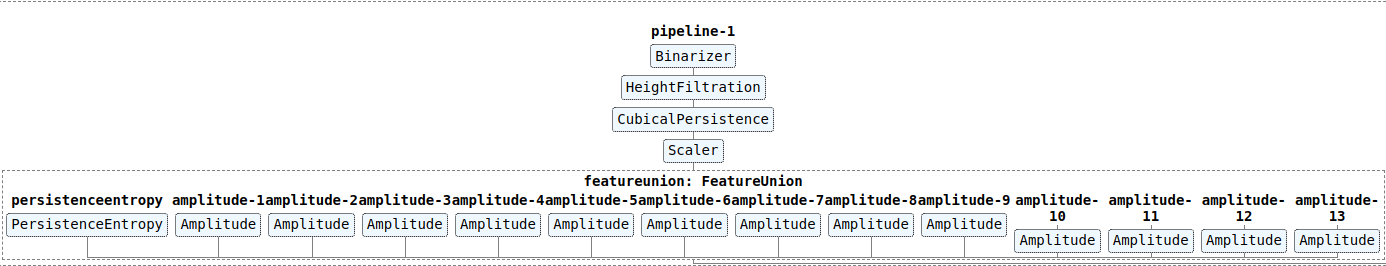
\includegraphics[width=\textwidth]{pipelineDiagram.png}\\
		\caption{Алгоритм получения признаков для Height Filtration}
		\label{pipeline}
	\end{center}
\end{figure}

Опишем подробнее алгоритм получения признаков. Первым шагом является бинаризация изображения с заранее выбранным пороговым значением(в данной работе значение порога равнялось $0.4$). Это нужно для того, чтобы далее воспользоваться специальными методами фильтрации, которые работают именно с бинарным изображением. Бинарным изображением будет называть отображение $B: \mathbb{R}^d \to \{0, 1\}$.

Далее по бинарному изображению $B$ строятся специальные фильтрации. По большому счету фильтрации можно воспринимать как трансформации бинарного изображения обратно в черно-белое, пропущенное через специальный фильтр. Так как в результате получается черно-белое изображение, то можно считать устойчивые гомологии сразу для самой картинки, но обычно построение черно-белого изображения через бинаризацию и фильтрацию наиболее сильно подчеркивает различные топологические особенности. В данном алгоритме использовалась т.н. фильтрация по высоте, радиальная фильтрация, а также фильтрация по плотности(рис. \ref{filtration-comparison}). 

\begin{figure}[!htbp]
	\begin{center}
		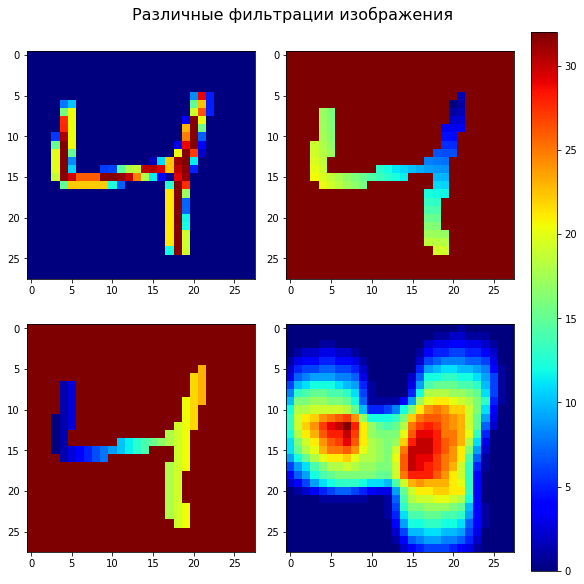
\includegraphics[width=0.75\textwidth]{differentFiltrations.png}\\
		\caption{Черно-белые изображения, полученные с помощью различных фильтраций. Для наглядности, была использована цветная гамма для представления черно-белых значений. В верхнем левом углу -- оригинальное изображение; в верхней правой -- радиальная фильтрация. В нижнем левой углу -- фильтрация по высоте; в нижнем правом углу -- фильтрация по плотности}
		\label{filtration-comparison}
	\end{center}
\end{figure}
Фильтрация по высоте(Height filtration) -- это отображение $H: I \to \mathbb{R}$, где $I$ -- это бинарное изображение в общем случае размерности $d$(в нашем случае размерность равна $2$), которое каждому пикселю изображения $p$ сопоставляет расстояние до гиперплоскости, которая определена вектором $v$ длины $1$, заданным заранее:
\[
H: p \mapsto 
	\left\{
		\begin{array}{ll}
			\langle p,v \rangle, & \text{если } B(p) = 1, \\
			H_\infty, & \text{иначе,}
		\end{array}
	\right.
\]
где $H_\infty$ -- это значение фильтрации $H$ самого дальнего пикселя изображения до гиперплоскости.

Радиальная фильтрация(Radial filtration) -- это отображение $R: I \to \mathbb{R}$, которое каждому пикселю изображения сопоставляет расстояние до выбранного заранее центра $c$:
\[
	R: p \mapsto 
		\left\{
			\begin{array}{ll}
				\norm{c - p}_2, & \text{если } B(p) = 1, \\
				R_\infty, & \text{иначе,}
			\end{array}
		\right.
\]
где $R_\infty$ -- это расстояние самого дальнего пикселя до центра. То есть фильтрация строится исходя из значения некоторой радиальной функции от пикселя $p$, у которого $B(p)=1$.

Фильтрация по плотности(Density filtration) -- это отображение $D: I \to \mathbb{R}$, которое каждому пикселю изображения сопоставляет число пикселей $p$, таких, что $B(p)=1$, находящихся на растоянии не больше задаваемого $r$:
\[
	D_r(p) \coloneqq \abs{\{ v \in I | B(v) = 1 \land \norm{p-v} \leq r \}},
\]
где $\norm\cdot$ -- любая норма в $\mathbb{R}^2$. В данном алгоритме использовалась стандартная евклидова метрика.

Так как вектор направления для фильтрации по высоте и центр для радиальной фильтрации задается заранее, то можно формировать различные фильтрации при различных значениях вектора направления и центра. В данном алгоритме фильтрация по высоте строилась с $8$ различными значениями для вектора направления, радиальная фильтрация строилась с $9$ различными значениями для центра, а фильтрация по плотности строилась с $3$ различными значениями для радиуса. Таким образом, для одного изображения получалось $20$ фильтрации.

\begin{figure}[!htbp]
	\begin{center}
		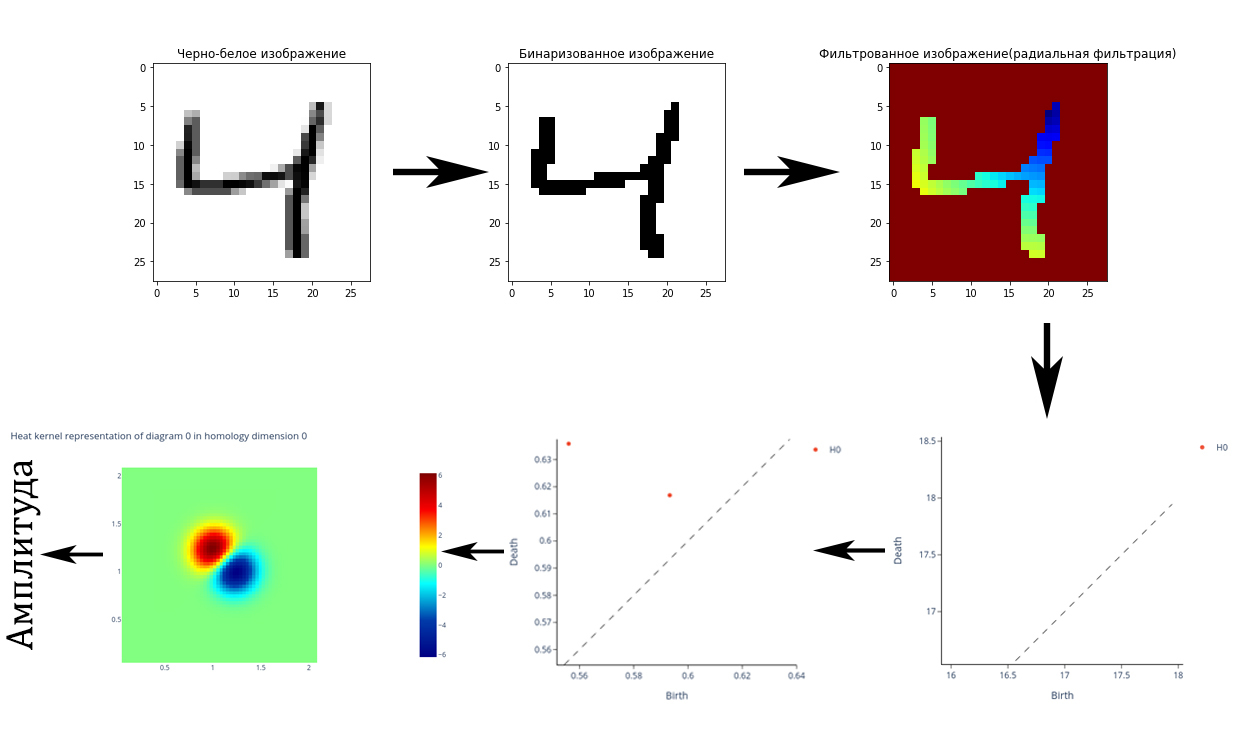
\includegraphics[width=0.75\textwidth]{pipe.jpg}\\
		\caption{Пример работы алгоритма}
		\label{example}
	\end{center}
\end{figure}

Далее для каждой из полученных фильтраций вычислялись устойчивые гомологии $0$ и $1$ размерности, а по ним строились диаграммы персистентности, которые далее были приведены к одному и тому же масштабу. 

\begin{figure}[!htbp]
	\begin{subfigure}{.33\textwidth}
		\centering
		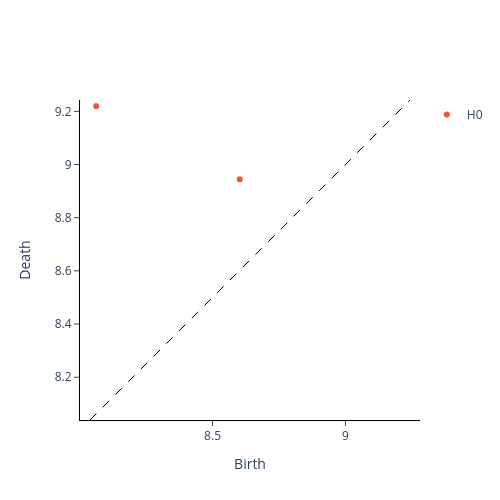
\includegraphics[width=\linewidth]{radial_persistence.png}\\
		\caption{Radial Filtration}
	\end{subfigure}%
	\begin{subfigure}{.33\textwidth}
		\centering
		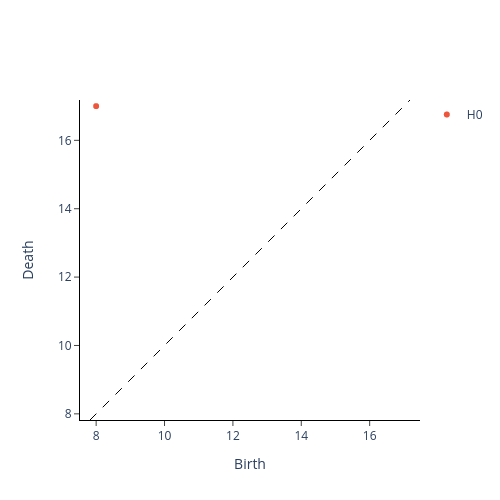
\includegraphics[width=\linewidth]{height_persistence.png}\\
		\caption{Height Filtration}
	\end{subfigure}%
	\begin{subfigure}{.33\textwidth}
		\centering
		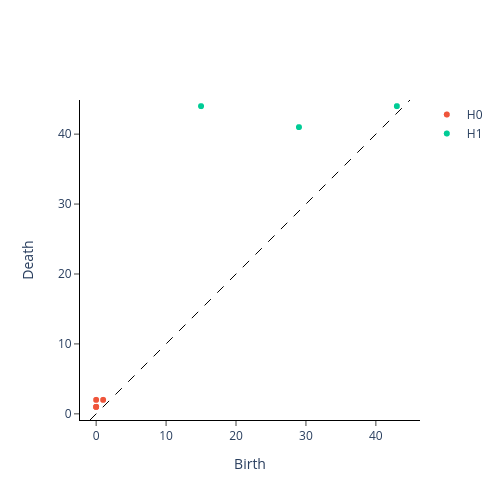
\includegraphics[width=\linewidth]{density_persistence.png}\\
		\caption{Density Filtration}
	\end{subfigure}%
	\caption{Диаграммы устойчивости для различных фильтраций}
	\label{persistences}
\end{figure}

 На рис. \ref{example} представлен пример работы алгоритма для одного бинарного изображения из датасета. На рис. \ref{persistences} представлены диаграммы устойчивости для различных фильтраций. На рис. \ref{scaled_persistences} представлены диаграммы устойчивости, приведенные к одному и тому же масштабу. Видно, что изменились значения шкал рождения/смерти у диаграмм.


\begin{figure}[!htbp]
	\begin{subfigure}{.33\textwidth}
		\centering
		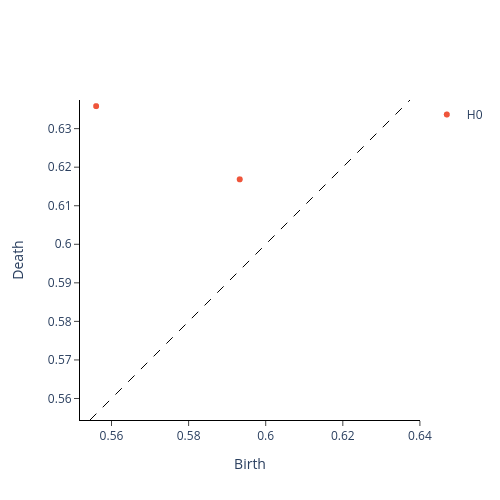
\includegraphics[width=\linewidth]{scaled_radial_persistence.png}\\
		\caption{Radial Filtration}
	\end{subfigure}%
	\begin{subfigure}{.33\textwidth}
		\centering
		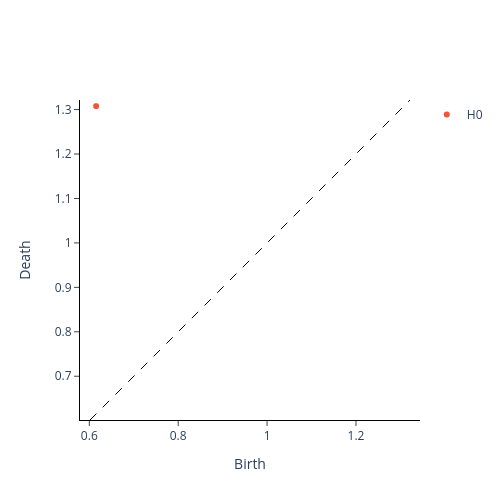
\includegraphics[width=\linewidth]{scaled_height_persistence.png}\\
		\caption{Height Filtration}
	\end{subfigure}%
	\begin{subfigure}{.33\textwidth}
		\centering
		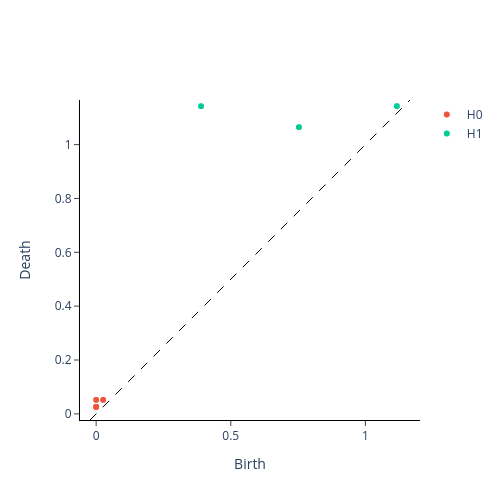
\includegraphics[width=\linewidth]{scaled_density_persistence.png}\\
		\caption{Density Filtration}
	\end{subfigure}%
	\caption{Диаграммы устойчивости для различных фильтраций, приведенные к одному масштабу}
	\label{scaled_persistences}
\end{figure}

В свою же очередь, для каждой диаграммы вычислялись $14$ признаков: персистентная энтропия и $13$ амплитуд для различных векторных представлений. На рис. \ref{representations} представлен пример таких представлений для различных фильтраций. Таким образом, для одной картинки получалось $20 \times 2 \times 14 = 560$ признаков. Однако вероятно, что некоторые из таких признаков будут коррелировать, а поэтому необходимо будет произвести отбор признаков.

\begin{figure}[!htbp]
	\begin{subfigure}{.33\textwidth}
		\centering
		
\includegraphics[width=\linewidth]{heat_height.png}\\
		\caption{Height filtration}
	\end{subfigure}%
	\begin{subfigure}{.33\textwidth}
		\centering
		
\includegraphics[width=\linewidth]{heat_rad.png}\\
		\caption{Radial filtration}
	\end{subfigure}%
	\begin{subfigure}{.33\textwidth}
		\centering
		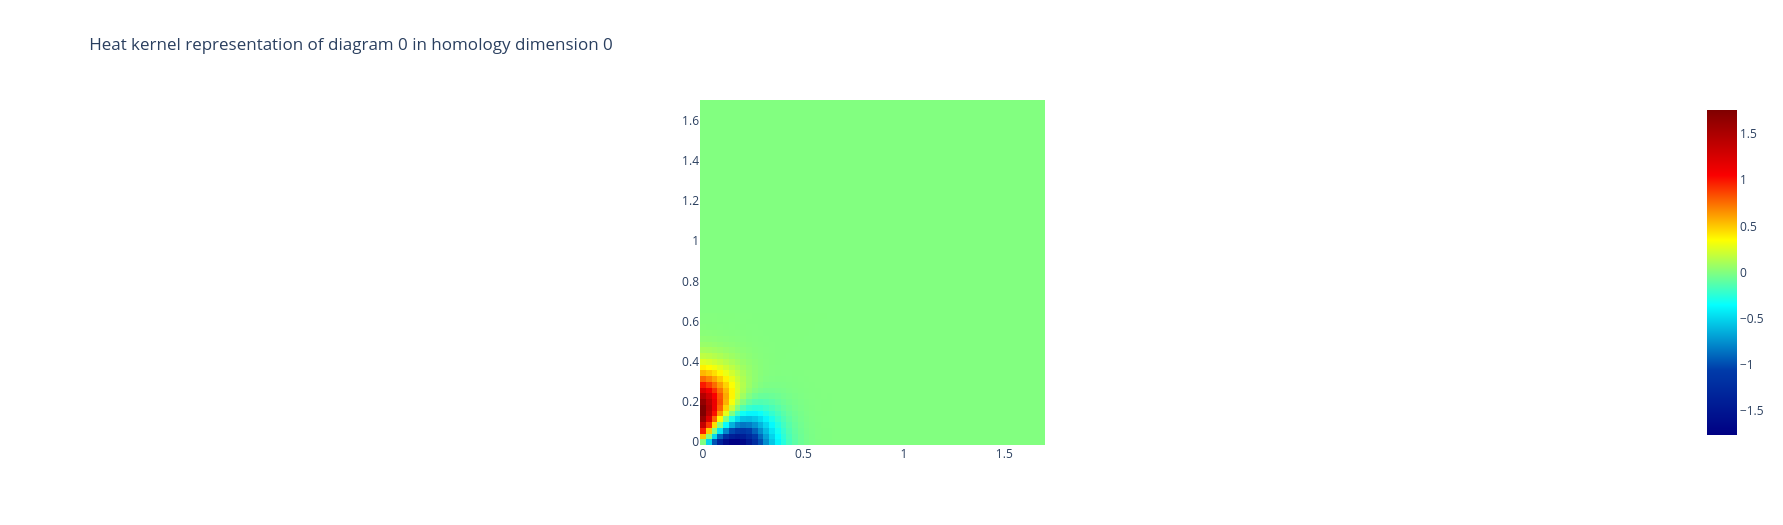
\includegraphics[width=\linewidth]{heat_dense.png}\\
		\caption{Density filtration}
	\end{subfigure}%
	\caption{Heat Kernel для различных фильтраций для одного и того же изображения}
	\label{representations}
\end{figure}

После получения векторного представления для изображений из выборки, дальнейшим этапом является обучение модели машинного обучения. В данной работе использовались следующие модели:
\begin{itemize}
	\item Метод опорных векторов
	\item Случайный лес
	\item Логистическая регрессия
	\item LightGBM
	\item CatBoost
	\item XGBoost
\end{itemize}
Первым шагом было запустить эти модели без настраивания параметров и отбора признаков, и посмотреть, как хорошо они справляются с задачей, т.е. таким образом получить начальное значение для каждой из модели, чтобы в дальнейшем значения качества моделей увеличивать как за счет настраивания параметров модели, так и за счет отбора признаков. Получившиеся результаты отображены в табл. \ref{tabl:baselines}

\begin{table}[!htbp]
	\centering
	\small
	\begin{tabularx}{\linewidth}{|X|X|X|}
		\hline
		Название модели & Значение на тренировочной выборке & Значение на тестовой выборке\\ \hline
		Логистическая регрессия & 0.989 & 0.903 \\
		\hline 
		Метод опорных векторов & 1.0 & 0.893 \\
		\hline
		Случайный лес & 1.0 & 0.89 \\
		\hline
		LightGBM & 1.0 & 0.9 \\
		\hline
		XGBoost & 1.0 & 0.883 \\
		\hline
		CatBoost & 1.0 & 0.893 \\ 
		\hline
	\end{tabularx}
	\caption{Значения базовых моделей на тренировочной и тестовой выборках}	
	\label{tabl:baselines}
\end{table}

Несмотря на очевидное переобучение -- значения на тренировочной выборке куда лучше, чем на тестовой -- все модели проявили себя очень хорошо и показали неплохие результаты(тут стоит отметить, что современные сверточные нейронные сети достигают $99.95\%$ точности). Попробуем для каждой модели сделать поиск по сетке, чтобы улучшить результаты моделей. Результат поиска по сетке представлен в табл. \ref{tabl:gridsearch}. Можно заметить, что для некоторых моделей проблема переобучения исчезла в результате подбора параметров.

\begin{table}[!htbp]
	\centering
	\small
	\begin{tabularx}{\linewidth}{|X|X|X|}
		\hline
		Название модели & Значение на тренировочной выборке & Значение на тестовой выборке\\ \hline
		Логистическая регрессия & 0.911 & 0.917 \\
		\hline 
		Метод опорных векторов & 0.903 & 0.893 \\
		\hline
		Случайный лес & 0.88 & 0.87 \\
		\hline
		LightGBM & 1.0 & 0.9 \\ %CHANGE
		\hline
		XGBoost & 1.0 & 0.883 \\ %CHANGE
		\hline
		CatBoost & 1.0 & 0.893 \\ 
		\hline
	\end{tabularx}
	\caption{Значения наилучших моделей, полученных в результате подбора параметров поиском по сетке, на тренировочной и тестовой выборках}	
	\label{tabl:gridsearch}
\end{table}

Как было сказано ранее, скорее всего многие признаки коррелируют между собой. Поэтому дальнейший шаг -- это отбор признаков. Сперва убедимся, что уменьшение признаков может привести к росту качества модели. Для этого запустим случайный лес на выборке. Случайный лес может быть использован в качестве отбора признаков -- есть возможность подсчитать важность признаков для этой модели. Те признаки, которые оказались наиболее важны для случайного леса, вероятно будут и наиболее важными и для других моделей. Поэтому с помощью случайного леса упорядочим все признаки по убыванию их важности. Далее в цикле будем запускать модели на выборке, но с разным числом признаков -- так как они упорядочены, то будем брать первые $50n$ признаков, где $1 \leq n \leq 11$. Запускать модели будем с поиском по сетке, чтобы использовать наилучшие параметры для данной выборке. График зависимости качества построенных моделей от числа признаков представлен на рис. \ref{accuracy-numFeatures}.

\begin{figure}[!htbp]
	\begin{center}
		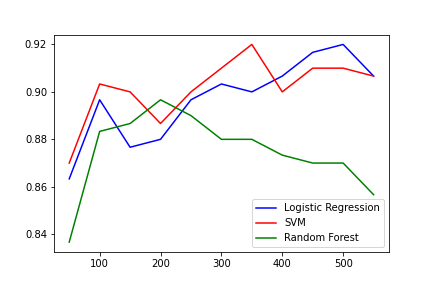
\includegraphics[width=0.75\textwidth]{models-topfeatures.png}\\
		\caption{График зависимости качества построенных моделей от числа признаков}
		\label{accuracy-numFeatures}
	\end{center}
\end{figure}

На графике видно, что, уменьшив количество признаков, все модели улучшают свои показатели качества. 

Далее можно сравнить качество моделей, которые используют топологические признаки, с качеством моделей, которые в качестве признаков будут получать просто векторное представление изображения. То есть для таких моделей признаками будут сами значения пикселей изображения. Так как модели с топологическими признаками показали наилучший результат именно при уменьшении количества признаков, то также отсортируем признаки для новых моделей по убыванию важности для случайного леса, и будем брать первые $50n$ признаков, каждый раз обучая модель с поиском по сетке, чтобы подобрать наилучшие параметры. Так как теперь признаков будет $28 \times 28 = 784$, то $1 \leq n \leq 15$. На графике \ref{accuracies_diff_features} представлены сравнения различных моделей, но с разными признаками. 

\begin{figure}[!htbp]
	    \centering % <-- added
	\begin{subfigure}{0.25\textwidth}
		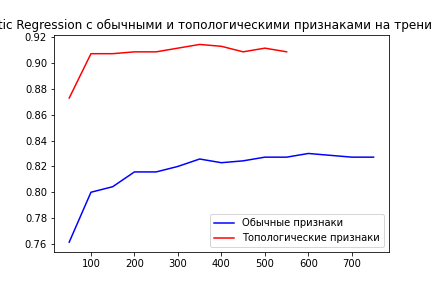
\includegraphics[width=\linewidth]{log_diff_features_train.png}
		\caption{Логистическая регрессия на тренировочной выборке}
		\label{fig:1}
	\end{subfigure}\hfil % <-- added
	\begin{subfigure}{0.25\textwidth}
		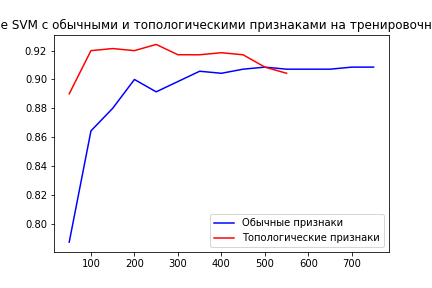
\includegraphics[width=\linewidth]{svm_diff_features_train.png}
		\caption{Метод опорных векторов на тренировочной выборке}
		\label{fig:2}
	\end{subfigure}\hfil % <-- added
	\begin{subfigure}{0.25\textwidth}
		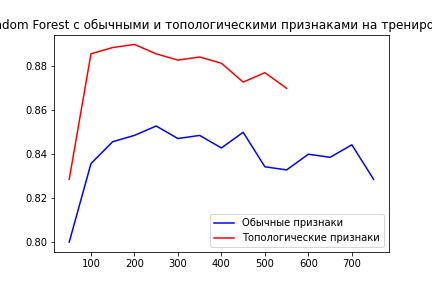
\includegraphics[width=\linewidth]{rf_diff_features_train.png}
		\caption{Случайный лес на тренировочной выборке}
		\label{fig:3}
	\end{subfigure}
	
	\medskip
	\begin{subfigure}{0.25\textwidth}
		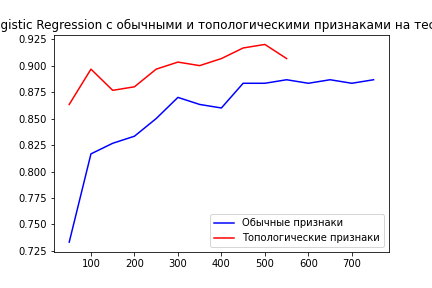
\includegraphics[width=\linewidth]{log_diff_features_test.png}
		\caption{Логистическая регрессия на тестовой выборке}
		\label{fig:4}
	\end{subfigure}\hfil % <-- added
	\begin{subfigure}{0.25\textwidth}
		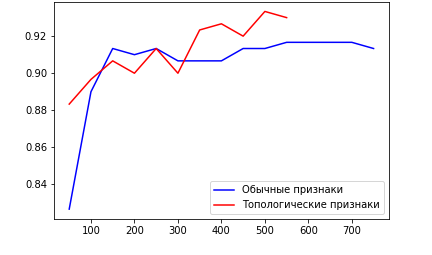
\includegraphics[width=\linewidth]{svm_diff_features_test.png}
		\caption{Метод опорных векторов на тестовой выборке}
		\label{fig:5}
	\end{subfigure}\hfil % <-- added
	\begin{subfigure}{0.25\textwidth}
		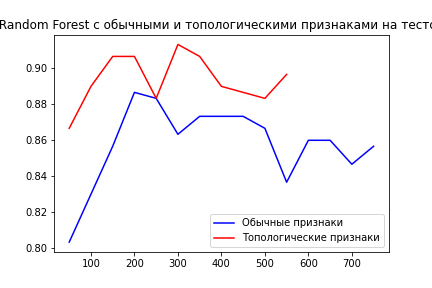
\includegraphics[width=\linewidth]{rf_diff_features_test.png}
		\caption{Случайный лес на тестовой выборке}
		\label{fig:6}
	\end{subfigure}
	\caption{Сравнение различных моделей, которые используют различные признаки}
	\label{accuracies_diff_features}
\end{figure}

Видно, что модели с топологическими признаками при малом количестве признаков достигает лучшей точности. Отсюда можно сделать вывод, что топологические признаки содержат в себе наиболее важную, релевантную информацию о структуре данных в меньшем числе признаков. Поэтому такой подход можно рассматривать как подход для уменьшения размерности данных. 

\begin{figure}[!htbp]
	\begin{center}
		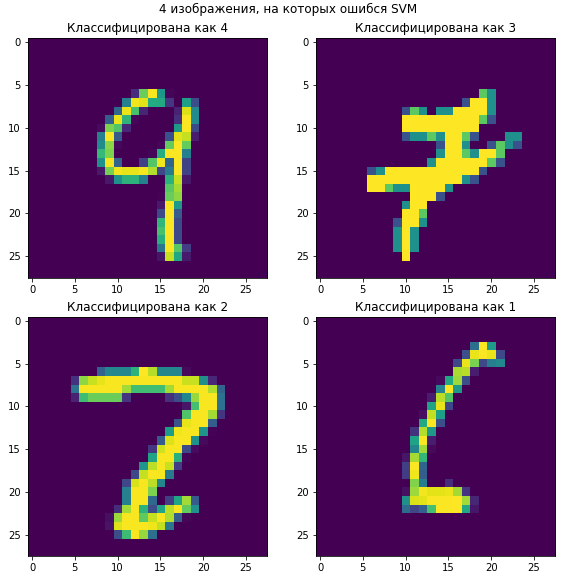
\includegraphics[width=0.75\textwidth]{missclassified.png}\\
		\caption{Первые несколько изображений, на которых ошибся классификатор}
		\label{missclassified}
	\end{center}
\end{figure}


Видно, что метод опорных векторов с подобранными параметрами на 400 лучших признаках, отобранных с помощью случайного леса, показывает чуть ли не самый высокий результат. Интересно посмотреть, на каких изображений эта модель ошиблась. На рис. \ref{missclassified} представлены как раз такие 4 изображения. Видно, что цифры, на которых ошибся классификатор, действительно похожи на те, которые классификатор предписал данным изображениях.

	
	\section{Заключение}
Перекати поле ...
%\bibliography{outro/resources}
%\begin{thebibliography}{99}
	\bibitem{Viro}
	Виро О.Я., Иванов О.А., Нецветаев Н.Ю., Харламов В.М. (2018). Элементарная топология. 978-5-4439-2680-3.
	\bibitem{Vick}
	Вик Дж. У. (2005). Теория гомологий. Введение в алгебраическую топологию. 5-94057-086-0.
	\bibitem{Hatcher}
	Хатчер А. (2011). Алгебраическая топология. 978-5-94057-748-5.
	\bibitem{Munkres}
	Munkres, James R. (2000). Topology. 0-13-181629-2.
	\bibitem{MathAndMyth}
	Фоменко А.Т. (2001). Математика и миф сквозь призму геометрии. URL: \url{http://dfgm.math.msu.su/files/fomenko/myth-vved.php}
	\bibitem{Edelsbrunner et al}
	Edelsbrunner, H., Letscher, D., and Zomorodian, A. (2002). Topological persistence and simplification. Discrete Comput. Geom., 28:511–533.
	\bibitem{Carlsson and Zomorodian}
	Zomorodian, A. and Carlsson, G. (2005). Computing persistent homology. Discrete Comput.
	Geom., 33(2):249–274.
	\bibitem{Carlsson}
	Carlsson, G. (2009). Topology and data. AMS Bulletin, 46(2):255–308.
	\bibitem{Fasy et al}
	Brittany T. Fasy, Jisu Kim, Fabrizio Lecci, Clement
	Maria, David L. Millman, and Vincent Rouvreau. Introduction to the R package TDA. URL: \url{https://cran.r-project.org/web/packages/TDA/vignettes/article.pdf}
		\bibitem{base}
	F. Chazal An introduction to Topological Data Analysis: fundamental and practical aspects for data scientists / F.Chazal, B. Michel. URL : \url{https://arxiv.org/pdf/1710.04019.pdf}
	
	\bibitem{Edelsbrunner}
	H. Edelsbrunner Computational Topology An Introduction / H. Edelsbrunner, J. Harer ; AMS : Providence, 2009. -- 241 с.
	
	\bibitem{Zomorodian} 
	A. Zomorodian Computing persistent homology / A. Zomorodian, G. Carlsson // Discrete Comput. Geom. -- 2005. -- Vol. 33, № 2. -- P. 249 -- 274. URL : \url{https://geometry.stanford.edu/papers/zc-cph-05/zc-cph-05.pdf}
	
	\bibitem{alsobase}
	N. Otter A roadmap for the computation of persistent homology / N. Otter, M.A. Porter, U. Tillmann, P. Grindrod, H. A Harrington // EPJ Data Sci. -- 2017. -- Vol. 6, №17. URL : \url{https://epjdatascience.springeropen.com/articles/10.1140/epjds/s13688-017-0109-5}
	
	\bibitem{giotto}
	Giotto-tda -- библиотека для топологического анализа данных на Python. -- URL : \url{https://github.com/giotto-ai/giotto-tda}
	
	\bibitem{gudhi}
	GUDHI -- библиотека для топологического анализа данных на C++ с интерфейсом для Python. -- URL : \url{https://gudhi.inria.fr/}
	
	\bibitem{modules}
	F. Chazal The Structure and Stability of Persistence Modules / F. Chazal, V. de Silva, M. Glisse, S. Outdot. URL : \url{https://arxiv.org/pdf/1207.3674.pdf}
	
	\bibitem{dionysus}
	Dionysus 2 -- библиотека для вычислений устойчивых гомологий, написанная на C++ и имеющая интерфейс на Python. URL : \url{https://www.mrzv.org/software/dionysus/}
	
	\bibitem{Tadasets}
	Tadasets -- библиотека, содержащая синтетические датасеты для топологического анализа данных. URL : \url{https://github.com/scikit-tda/tadasets}
	
	\bibitem{Ripser}
	Интерфейс для Ripser на Python. URL : \url{https://ripser.scikit-tda.org/en/latest/}
	
	\bibitem{scikit}
	Scikit-TDA -- библиотека для топологического анализа данных, содержащая Ripser и Tadasets. URL : \url{https://scikit-tda.org/}
	
	\bibitem{colab}
	Google Colab -- Сервис Google, предоставляющий возможность запускать код, написанный на Python, в браузере, обладающий интерфейсом Jupyter Notebook, специально созданный для задач машинного обучения, анализа данных, а также образования. URL : \url{https://colab.research.google.com/}
	
	\bibitem{twist}
	C. Chen Persistent Homology Computation with a Twist / C. Chen, M. Kerber // EuroCG -- 2011. URL : \url{https://eurocg11.inf.ethz.ch/abstracts/22.pdf}
	
	\bibitem{multifield}
	J. Boissonnat Computing Persistent Homology with Various Coefficient Fields in a Single Pass / J.Boissonnat, C. Maria. URL : \url{https://arxiv.org/abs/2001.02960}.
	
	\bibitem{zigzag}
	C. Maria Computing Persistent Cohomology / C. Maria, S. Oudot. URL: \url{https://arxiv.org/abs/1608.06039}.
	
\end{thebibliography}
	
	\newpage  
	\nocite{*}
	\printbibliography[title={Список использованных источников}]
	\addcontentsline{toc}{chapter}{Список использованных источников}
	\newpage
	\chapter*{Приложение 1 Код сравнения методов на топологических и обычных признаках}
	\addcontentsline{toc}{chapter}{Приложение 1 Код сравнения методов на топологических и обычных признаках}
	\lstinputlisting{listing.py}
\end{document}